\documentclass[acmtog, screen, balance]{acmart}
\usepackage[htt]{hyphenat}
\usepackage{graphicx}
\usepackage{lipsum}
\usepackage{pgfgantt}
\usepackage{enumitem}
\usepackage{booktabs}
\usepackage{fontawesome5}
\usepackage{listings}
\usepackage{minted}
\usepackage{xcolor}

\newlist{questions}{enumerate}{2}
\setlist[questions,1]{label=\textbf{RQ\arabic*.},ref=RQ\arabic*}
\setlist[questions,2]{label=(\alph*),ref=\thequestionsi(\alph*)}
\graphicspath{{images/}}

\AtBeginDocument{%
  \providecommand\BibTeX{{%
    \normalfont B\kern-0.5em{\scshape i\kern-0.25em b}\kern-0.8em\TeX}}}

% \setcopyright{cc}
\copyrightyear{2023}
\acmYear{2023}

\acmConference[TScIT 39]{39$^{th}$ Twente Student Conference on IT}{July 7,
  2023}{Enschede, The Netherlands}
\acmDOI{}
\acmISBN{}

\begin{document}

\title{Satellite to Radar: Sequence to Sequence Learning for precipitation nowcasting}

\author{Mark Bruderer}
\email{m.a.bruderervanblerk@student.utwente.nl}
\affiliation{%
  \institution{University of Twente}
  \streetaddress{P.O. Box 217}
  \city{Enschede}
  \country{The Netherlands}
  \postcode{7500AE}
}

\renewcommand{\shortauthors}{Mark Bruderer}

\begin{abstract}
\section*{Abstract}
The forecasting of rain is a complex problem with centuries of scientific work.
The implications of weather for individuals and companies continue to be important.
Machine Learning approaches have been shown to outperform state of the art physics based models of weather for short term predictions.
Using multi-spectral satellite images as out input and radar reflectivity as the target.  
We investigate three different types of models: 3D U-Net, ConvLSTM and ConvLSTM with self attention.
We found that ConvLSTM outperforms the other approaches for both classification and regression pixel rain intensities.
\end{abstract}

\keywords{Machine Learning, Sequence to Sequence, Radar, Satellite, Storms, Forecasting, 3D U-Net, ConvLSTM, Attention Mechanism}

\settopmatter{printacmref=false}


\begin{teaserfigure}
    \renewcommand{\thefootnote}{\arabic{footnote}}
    \includegraphics*[width=\textwidth, trim=0in 0.0in 0in 16.0in]{images/lightning.jpg}
    \caption{A supercell thunderstorm at twilight in SW Oklahoma.\protect\footnotemark}
    \Description{A supercell thunderstorm at twilight in SW Oklahoma.}
    \label{fig:teaser}
\end{teaserfigure}

\maketitle

\footnotetext[1]{Photograph by \href{https://unsplash.com/@raychelsnr}{Raychel Sanner}, \href{https://unsplash.com/license}{Unsplash Licence}}

\section{Introduction} \label{introduction}
Precipitation forecasting is essential to reduce the risk of life threatening situations. Different types of rainfall ranging from mist to heavy rain have a major impact for different societal sectors including agriculture, aviation, outdoor events, and the energy industry.
By having timely and accurate predictions of rainfall which in turn indicate the potential for destructive storms we can prevent injuries, assist companies in predicting energy production and use resources efficiently.
\medskip

A particularly strong threat is posed by rain storms and thunderstorms. Storms are one of the most destructive weather events in nature, capable of destroying human structures and even lead to loss of life \cite{noaa-national-severe-storms-laboratory-no-date}. Predicting storms is crucial and presents it's own set of challenges.
\medskip

At present meteorologists are able to successfully predict many instances of precipitation. Techniques that are used in practice range from manual analysis of current weather data (e.g radar or satellite images) to complex physics based simulations of our atmosphere with Numerical Weather Prediction (\textsc{NWP}) models.
Various short term forecasting methods are based on \textit{optical flow}. Optical flow functions in two steps, first cumulonimbus (storm) clouds are identified, and then their movement is tracked to predict the location of precipitation. Thus in this case, the forming and dissipation of clouds known as a \textit{cell-lifecycle} \cite{noaas-national-weather-service-no-date} is not taken into account \cite{prudden2020review}.
\medskip

Machine Learning (\textsc{ML}) approaches have also been developed to predict precipitation.
An improvement of machine learning models over \textsc{NWP} models is that they are much faster to produce predictions, thus ML models are more suitable for real-time or near-real-time predictions, such as required in disaster response and energy management. These short term predictions are referred to as \textit{nowcasts}. According to the universal approximation theorem \cite{cybenko-1989}, deep neural networks have the property of being able to approximate any function provided they have the correct weights, thus it is suggested that machine learning models can incorporate sources of predictability beyond optical flow such as the \textit{cell-lifecycle}.
Other suggested sources of predictability are: the elevation of terrain, convergence lines and the current time among others \cite{prudden2020review}.
\medskip

Thus far most machine learning approaches for precipitation nowcasting have focused on predicting future frames of currently available radar data \cite{shi2017deep, convlstm, rainet}. However taking this approach may eliminate the possibility of learning the \textit{cell-lifecycle}, due to the fact that the model only sees precipitation itself but not the cloud that is causing the precipitation.
\medskip


We propose to use multi-spectral satellite data to learn spatio-temporal mappings between sequences of satellite data and precipitation data in the near future. A well performing model could predict storm clouds when these clouds are still forming. An additional advantage is that contrary to radar data, satellite data is readily available over oceans and remote communities (See figure \ref{fig:radar-availability}) which allows for the prediction of precipitation over these regions.
\smallskip

\subsection{Problem Formulation}
We consider precipitation nowcasting as a self-supervised problem. In self-supervised tasks, explicit labels are not provided, but rather we can derive labels from the raw data itself, which is often the case with time-series data. Consequently, we can utilize established techniques in supervised learning to address our research problem. The prediction of labels can be accomplished through two approaches: predicting discrete classes that correspond to different rain intensity intervals, or conducting pixel-level regression to learn the precise values of precipitation.

\subsubsection{Regression Formulation} Consider a dataset \{X, Y\} consisting of pairs of input-output sequences indexed by $i \in \mathbb{N}$,
%where each input sequence represents a temporal sequence of $t$ satellite images with height $H$, width $W$ and $c$ channels.
Let $$X = \{x^{(i)} \in \mathbb{R}^{t \times h \times w \times c}\} \forall i$$ 
where $x^{(i)}$ is a tensor of dimension $t \times h \times w \times c$ representing the sequence of satellite images at position $i$, having $t$ time-steps, $h$ height, $w$ width and $c$ channels.
The set of output sequences is denoted as $$Y = \{y^{(i)} \in \mathbb{R}^{w\times h}\}\forall i$$
where $y^{(i)}$ represents the $i^{th}$ $h \times w$ dimensional tensor with each pixel being a real number collected by the radar reflectivity reading.
Here the width and height are the same as in the input sequence.
The problem is formulated as finding a function f(x). This function must minimize a chosen distance function $\mathcal{D}$ as follows:
Let $\hat{Y} = \{p(x^{(i)})\}\forall i$, representing the predicted outputs for each sequence of satellite images and identical in dimensions to $y^{(i)}$.
find f(x) such that $\mathcal{D}(\hat{Y}, Y)$ is minimized.

\subsubsection[short]{Classification Formulation}
Consider a dataset \{X, Y\} consisting of pairs of input-output sequences indexed by $i \in \mathbb{N}$,
%where each input sequence represents a temporal sequence of $t$ satellite images with height $H$, width $W$ and $c$ channels.
Let $$X = \{x^{(i)} \in \mathbb{R}^{t \times h \times w \times c}\} \forall i$$ 
where $x^{(i)}$ is a tensor of dimension $t \times h \times w \times c$ representing the sequence of satellite images at position $i$, having $t$ time-steps, $h$ height, $w$ width and $c$ channels.
The set of output sequences is denoted as $$Y = \{y^{(i)} \in \mathbb{N}^{w\times h}\}\forall i$$
where $y^{(i)}$ represents the $i^{th}$ h $\times w$ dimensional tensor containing discrete integers mapping to rainfall intensity classes.
The problem is formulated as finding a probability mass function p(x). This function must minimize the Cross Entropy Loss expressed as follows:

$$E = \frac{1}{h+w}\sum_{i=1}^h\sum_{j=1}^w t_{ij} log(p_{ij})$$

Let $\hat{Y} = \{p(x^{(i)})\}\forall i$, representing the predicted outputs for each sequence of satellite images and identical in dimensions to $y^{(i)}$.
find p(x) such that $E(\hat{Y}, Y)$ is minimized.

\subsection{Research Question}
\textbf{RQ}: \textit{How can a deep learning model be trained to predict radar data with multi-spectral satellite data ?}
\smallskip

This research question will be answered by looking at the following sub research questions:
\begin{enumerate}
    \item \textit{how must data be preprocessed and aggregated to create a model capable of predicting precipitation based on satellite data?}
    \item \textit{How can the process of training be simplified to be able to experiment with different architectures ?}
    \item \textit{what model architecture performs the best based on established metrics for classification and regression ?}
\end{enumerate}


\section{Contribution}
In this research we focus on testing the hypothesis if a model trained on satellite sequences is capable of forecasting precipitation.
This is unclear as of now because most other studies rely on only radar or a combination of satellite and radar.
In the precipitation nowcasting field of research, there is a symbiosis between the task of video-to-video prediction and precipitation forecasting, models created for one are used in the other and vice-versa.
It is unclear whether these techniques can be successfully applied when using input and output data from different domains. We compare three different model architectures, UNet, ConvLSTM + Attention and ConvLSTM. All of these techniques are analyzed in both pixel-classification and pixel-regression implementations.

\section{Related Works}
In this section we will discuss the existing work in precipitation nowcasting via machine learning. This section is structured by the type of input data used in the approaches, first we list radar based learning and then we discuss satellite based approaches.

\subsection{Radar Based Nowcasting}

Recurrent neural networks (\textsc{RNNs}) have been created to learn temporal relationships in data, therefore they are a natural candidate to the task of learning spatio-temporal patterns of weather. The \textsc{LSTM} architecture was developed by Hochreiter and Schmidhuber \cite{lstm}, to solve the problem of vanishing and exploding gradients in RNNs and is widely used. Taking LSTM as a base and adapting the weights to kernels, \textsc{ConvLSTM} \cite{convlstm} was introduced for the task of precipitation nowcasting. Multiple layers of ConvLSTM are used in this paper to obtain a sequence to sequence architecture. A further improvement of ConvLSTM is \textsc{trajGRU} which was proposed by Shi et al. \cite{shi2017deep} to be able to learn the \textit{location-variant} structure for recurrent connections.
\smallskip

Pure convolutional neural networks have also been used to predict precipitation. As demonstrated by Bai et al. and Gering et al. \cite{bai2018empirical, gehring2017convolutional} convolutional neural architectures can outperform recurrent neural networks for a variety of sequence modelling tasks. This is the reason why many works on precipitation nowcasting have opted for pure convolutional networks \cite{rainet,agrawal2019machine}.
\smallskip

Due to machine learning models attempting to minimize loss, \textit{blurry predictions} can be produced by models. This can be alleviated by using generative models which sample from the possible futures and do not seek to provide a best average fit. Generative Adversarial Networks have been successfully applied to the task of precipitation nowcasting \cite{Ravuri_2021}.

\subsection{Satellite Based Nowcasting}

In their study Chen et al. built a \cite{precipitationEstimationFromSat} MLP to forecast radar data from satellite data. The researchers used a combination of low earth orbit satellite passive microwave and infrared channels from two different satellites. Their model is developed to predict up to 1.5 hours in the future by recursive predictions of the model.
\smallskip

A study that does not predict precipitation but uses lightning as a marker for extreme precipitation was performed by Brodehl et al. \cite{predictionLightning} this study uses a convolutional network to predict lightning events, and contributes the important observation that both the visual and infrared channels are important in differing ways to predict lightning.
\smallskip

The approach taken by the researchers of MetNet \cite{sønderby2020metnet} is to combine a convolutional block for spatial downsampling, then a ConvLSTM block for temporal encoding and finally a Axial attention block \cite{vaswani2017attention}. MetNet is able to perform more accurate forecasts than NWP models for up to 8 hours. In this study the input data that is used is both satellite and radar data as well as the elevation, time of the year and latitude and longitude values.

\section{Background}
In this section, we will explore the machine learning techniques utilized
in this study. Initially, we will delve into convolutional neural networks
(CNNs) and their advantages compared to multilayer perceptrons (MLPs).
Following the introduction of CNNs, we will focus U-Net a widely used fully convolutional network architecture.
Additionally, we will examine LSTM networks and their extension to ConvLSTM that incorporates convolutions.
\medskip

\subsection{Convolutional Neural Networks}

Convolutional neural networks (CNNs) were initially introduced by Yann LeCun in 1998 and applied to the challenge of handwritten digit classification \cite{lecun-1998}. However, the breakthrough for CNNs came later with the remarkable success achieved by Krizhevsky et al. in the ImageNet paper of 2012. This pivotal work revolutionized the field of image classification by significantly advancing the state of the art on the ImageNet dataset \cite{krizhevsky-2017}.

CNNs are a class of deep learning models strongly capable of solving computer vision tasks. Unlike fully connected neural networks, which treat input data as a one dimensional vector, CNNs are designed to process higher dimensional data such as images.
This distinction enables CNNs to exploit more spatial relationships and patterns in visual data as opposed to a flattened vector where these patters are not recoverable.

Additionally Convolutional neural networks reduce the amount of parameters that are needed for each layer. This reduction is caused by parameter sharing, in a
traditional multi-layer perceptron weights exist for each connection while in CNNs a set of kernels are applied to the input. The kernels used in CNNs are small and repeatedly applied across the input.
This reduces the amount of parameters the network has. 

\begin{figure}
  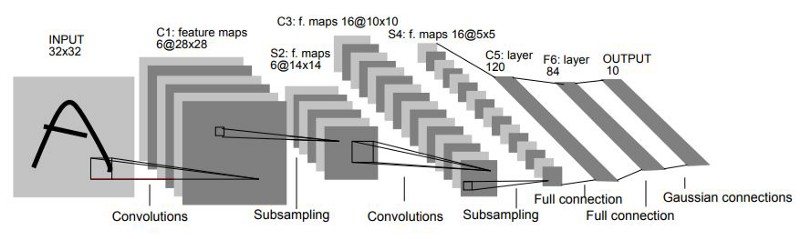
\includegraphics[width=8cm]{../images/cun.jpeg}
  \caption[short]{Architecture of LeNet-5: used for digit recognition and introduced by Yan LeCun \cite{lecun-1998}}
\end{figure}

\subsection{U-Net}
Semantic segmentation, the task of assigning a class label to each pixel in an image, is key to understand an image from a computer vision perspective.
This is the starting point for U-Net which was developed by Ronneberger et al. \cite{ronneberger-2015} to segment images from microscopes in biomedical applications.
U-Net is a fully convolutional architecture that provides accurate and detailed pixel-level predictions.
The U-Net architecture is specifically designed to capture both local and global context information.
The U-Net architecture gets its name from its U-shaped design (Figure \ref{fig:unet}), which consists of an encoder path and a decoder path.
The encoder path resembles a traditional CNN and serves to capture spatial information and learn feature representations at various scales.
It typically comprises multiple convolutional and pooling layers, where each convolutional layer extracts increasingly abstract features by convolving with learnable filters and applying non-linear activation functions.
The decoder path, on the other hand, aims to recover the spatial information lost during the pooling and down-sampling operations of the encoder.
It employs a series of upsampling and transposed convolutional layers to gradually increase the spatial resolution and reconstruct the detailed predictions.
The skip connections between the corresponding encoder and decoder layers help preserve fine-grained details and enable the fusion of local and global context information, facilitating more accurate segmentation.
These skip connections bridge the gap between low-level and high-level features, allowing the network to leverage both local and global context for precise pixel-wise predictions.
One of the key advantages of U-Net is its ability to capture contextual information effectively. By using skip connections, the network can combine low-level and high-level features, enabling the model to refine predictions by incorporating local details and global context simultaneously. This property is especially beneficial for tasks like semantic segmentation, where precise boundary delineation and accurate classification of object categories are essential.
\begin{figure}
  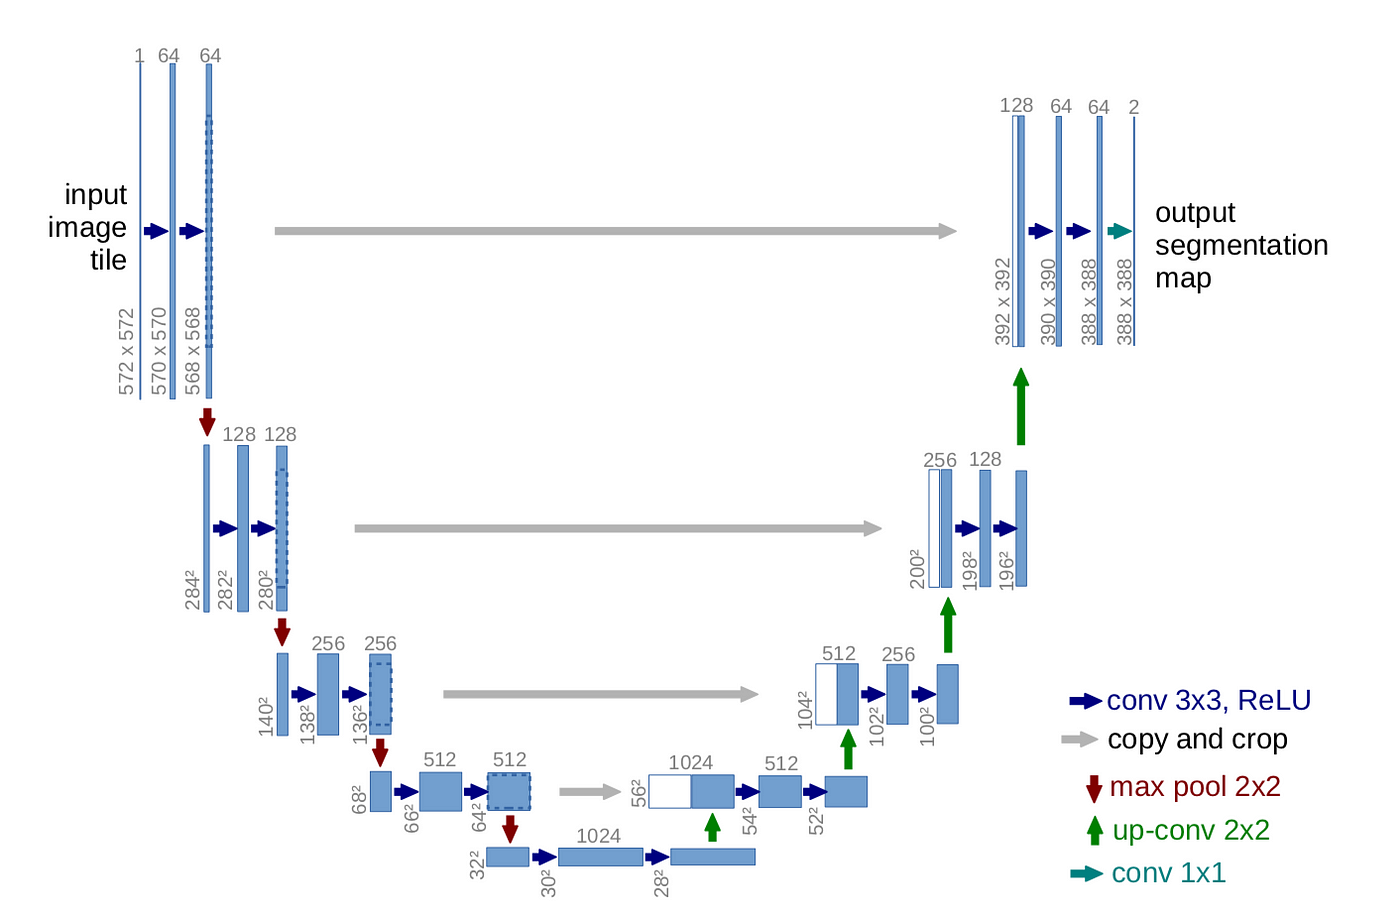
\includegraphics[width=8cm]{../images/unet.png}
  \caption[short]{U-Net}
  \label{fig:unet}
\end{figure}

\subsection{Convolutional LSTM}

\subsection{Attention}
Designed for machine translation Bahadanau et al. can be applied to sequence to sequence encoder decoder models.
how to pay the right amount of attention to the input sequence.

\section{Methodology}
In this section, we will provide explanations of the methods and techniques employed in our experiments.

\subsection{Engineering For Machine Learning}
In order to streamline our experimental process and minimize effort, we used specific tools and techniques to make
testing models more efficient.
We adopted the \texttt{zenml} \cite{zenml} framework to structure our training and preprocessing pipelines.
This framework brings several advantages to our workflow.
One notable benefit is the promotion of modularity in the design of our pipelines.
Each pipeline consists of individual steps, which enhances the code's modularity.
By defining a series of functions with clear inputs and outputs,
we ensure that each step can be easily understood and modified as needed.
Moreover, the \texttt{zenml} web application offers a convenient way to monitor the status of our pipelines.
This feature provides transparency and improves comprehension by providing insights into the outputs generated at each step.
For experiment tracking we used the \texttt{MLFlow} framework \cite{mlflow}.
This makes it easy to track all metrics over all experiments.
With \texttt{MLFlow} it is also possible to compare different parameters that were used during training to experimentally find the best combinations.
In \texttt{MLFlow} we save each finished model as an artifact which can be directly served as a server endpoint to start providing end users access to our models.
We used the pytorch lightning library. Using patterns such as the \texttt{DataModule} and {LightningModule} to accelerate the
research process. This library abstracts the process of backpropagation and updating parameters.
Furthermore pytorch ligthning \cite{lightning} handles
switching from training devices automatically for example \texttt{cpu} and \texttt{cuda} devices
which decouples the training code from specific hardware.
We made use of the \texttt{typed-settings} library \cite{typed} to allow cleanly structuring and validating settings for models.
This ensures that to train a new version of a model in most cases only adjustments to the configuration file needs to be done.
\texttt{typed-settings} supports passing training settings through toml configuration files, environment variables and command line options.

\subsection{Data Preprocessing}
For the preprocessing of data we created a pipeline which distinguishes between satellite images and radar images to process each following their own needs (See figure \ref{fig:preprocessing}).
\smallskip

The pipeline begins by obtaining all necessary files, from a remote storage bucket.
This is done by a Bucket Service class which uses the \texttt{boto3} \cite{boto}
library to interface with the bucket and download files in the required date ranges.
\smallskip

In the case of satellite data, the obtained files are compressed in zip files. The pipeline handles the extraction of these files deleting any files which are not needed along the way to ease the storage requirements.
Then we \textit{reproject} the satellite images using the \texttt{satpy} package. This downsampling is done by a combination of cropping and interpolation via the nearest-neighbor algorithm.
\smallskip

By reprojecting we reduce the dimensions of each satellite image to \texttt{256 x 256} pixels from it's original dimensions of \texttt{3712 x 3712}.
We also obtain only the geographical area of interest, specified by the coordinates for the lower corner \texttt{(50°0'0"N 0°0'0"E)} and the upper corner \texttt{(55°0'0"N 10°0'0"E)} of the region, this gives us
the area centered on the netherlands with other bordering countries (see figure \ref{fig:reprojection}). Additionally we change the map projection to \textit{Mercator} from the original \textit{Geostationary}.
This is done to have both input and target grids in the same map projections.
After reprojecting we perform a \textit{statistics} step where we aggregate the dataset by finding the minimum and maximum values for each channel see table \ref{tab:channels} for the list of all channels.
The statistics are necessary for the next step which is normalization. During the normalization step we perform the \textit{Min-Max} Normalization (equation 1).

\begin{figure}
  \centering
  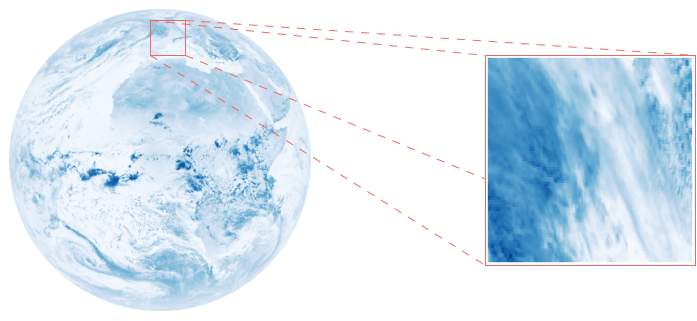
\includegraphics[width=225pt]{./images/reprored.png}
  \caption{Reprojection of Satellite Data: Converting from geostationary projection to mercator projection and reduce to area of interest.}
  \Description{Satellite Image of the earth}
  \label{fig:reprojection}
\end{figure}


\begin{equation}
  x_{normalized} = \frac{x-min(\bar{x})}{max(\bar{x})-min(\bar{x})}
\end{equation}

After finalizing the normalization step we sample an image from the dataset which is visualized to check for errors in the pipeline.
\smallskip

The radar pipeline begins with the downloaded \texttt{h5} files
each is converted to decibels relative to Z (dBZ) (equation 8) from a \textit{grayscale} unit ranging from 0 to 255.
Using decibels relative to Z adds to the interpretability  and makes it easier to weight loss functions and metrics
according to the level of precipitation. The drawback of this is that to plot the image or perform image transformations many
existing libraries make the assumption of either \textit{grayscale} or \textit{rgb} images, therefore to make use of these resources we must sometimes convert back to the \textit{grayscale} unit. 

\begin{equation}
  dBZ(x) = x \cdot 0.5 - 32
\end{equation}

The preprocessing pipeline then splits into two, one step will normalize values between 0 and 1 using \textit{Min-Max} normalization and the other step will use levels of \textit{dBZ} to create discrete ranges of precipitation to use as classes during training \ref{tab:classes}.
Finally the current images in the pipeline are resized using the nearest neighbor algorithm, to avoid changing the class values with bilinear interpolation.
Next identically to the satellite pipeline we sample and visualize a radar image for verification purposes.

\begin{figure}
  \centering
  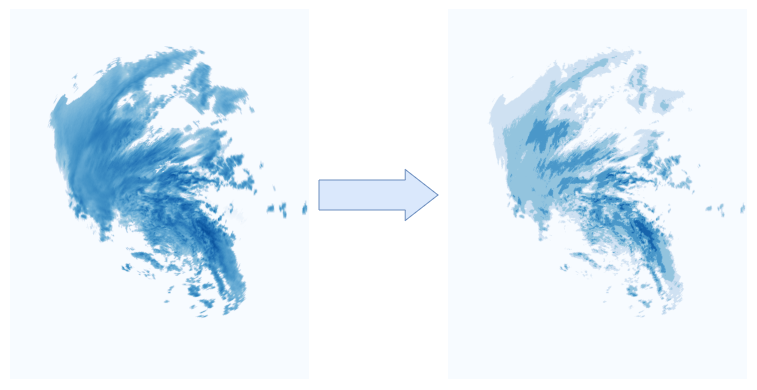
\includegraphics[width=225pt]{./images/bins.png}
  \caption{Preprocessed Radar Reflectivity Data For 2023-03-10 at 11:55 UTC. Left with normalized data and right with pixels put into 8 different rainfall intensity classes.}
  \Description{Satellite Image of the earth}
  \label{fig:bins}
\end{figure}


\begin{figure}
  \centering
  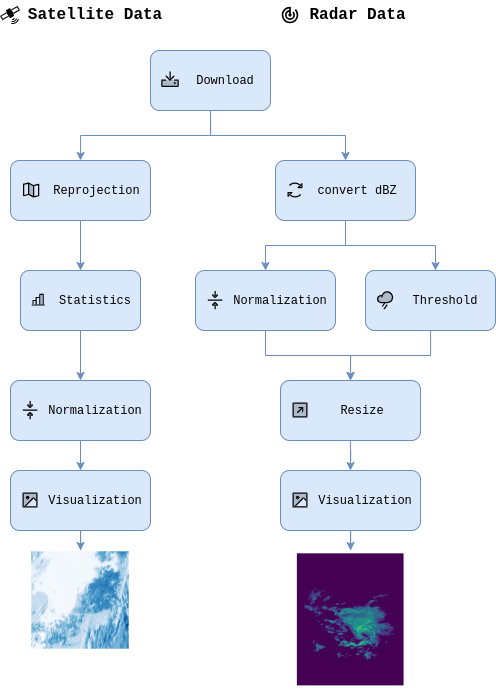
\includegraphics[width=225pt]{./images/prepro.png}
  \caption{Data Preprocessing Pipeline: Satellite Data and Radar data preprocessed separately}
  \Description{Satellite Image of the earth}
  \label{fig:preprocessing}
\end{figure}

\subsection{Proposed Model Architectures}
Three model architectures are tested: 3D U-Net, ConvLSTM and ConvLSTM with Attention Mechanism, all of these are suitable for classification and regression with a few alterations of the last layers.

The 3D U-Net based model is given a input patch of dimension $8\times11\times256\times256$. The U-Net model produces a segmented image for each slice of the depth dimension.
Therefore we added an additional 3D convolution after the normal U-Net architecture which reduces the output of the network from the shape $8\times8\times256\times256$ to the desired $1\times8\times256\times256$ or in the case of regression to $1\times256\times256$
\smallskip


For ConvLSTM models, we start with 3 layers of Convolutional LSTMs
with 64 filters that use a kernel size of 3.
Then the short term memory of the last layer is passed to three 2D Convolutional Layers.
The first Convolutional layer reduces the amount of channels to 32, the second to 16 and the last one to either 8 or 1 for classification and regression respectively.
In the intermediate layers a ReLU \cite{relu} activation function is performed.
\smallskip

The architecture of ConvLSTM with Attention Mechanism consists of 3 layers of Convolutional LSTMs,
with 64 filters with kernel size of 3. Then the short term memory of the last layer is passed to a Axial Positional Embedding Layer
and a single Axial Attention layer with 4 attention heads.  

\subsection{Experimental Setup}
We trained each model for 50 epochs. The batch size was set to 1 because of memory constraints. We used the \textsc{Adam} algorithm for optimization from Kingma et al \cite{kingma-2014}.
All model were trained on a single NVIDIA GeForce RTX 2070 SUPER GPU. We used different losses for classification and regression.
First we used Multi-Class CrossEntropyLoss for classification this first applies a log softmax activation function which normalizes the
outputs produced by our models. Then it calculates the cross entropy loss between the normalized input and the target.
For regression we used the MSE loss. To address class imbalance in the data we added weights for the CrossEntropyLoss. These weights were
obtained by finding the frequencies of the classes in the dataset as follows:

\begin{equation}
  weight(c) = 1 - \frac{1}{h\times w \times n} \times \sum_{i=1}^n \sum_{j=1}^h \sum_{k=1}^w [Y_{ijk} = c]
\end{equation}

We decided to conduct our experiments using $t = 5$, allowing for 1 hour and 15 minutes of temporal data, $h = 256$, $w = 256$, and $c = 12$.

We created 2 different types of datasets for use in the experiments.
The first type is a sequence dataset, this dataset does not repeat any satellite files. It increments the starting point at each sample
by the length of the satellite sequence. On the other hand to make use of all the available data we created a sliding sequence dataset which increments the starting point of the sequences by 1 meaning that the sequence moves by
1 satellite image forward. We have also handled aligning the satellite and corresponding radar target based on their timestamps. 

\subsection{Performance Evaluation}

To evaluate the performance of our models we implemented several metrics. Each of these metrics can be used to measure
the quality of a trained model. Utilizing a range of metrics allows us to better analyze the performance of a particular machine learning model.
Metrics that are used to measure the performance of classification problems are different from the metrics that are used for regression. Note that we
give the formulas that are used to calculate the metric for each image, in the reported results these metrics have been averaged over the entire test dataset.

\subsubsection{Regression Evaluation Metrics}
Regression metrics are often error functions, these functions calculate the distance between prediction and target values. 
When predicting more than one value, we can extend the definition of an error function
by calculating the mean or sum of all distances, the distances themselves are calculated with a certain distance metric for 2 values that are in the same position in the prediction and target.
This is an important distinction when considering that we predict a $h \times w$ image, to calculate the distance between the prediction and target, we will calculate the distance between each pixel then divide it by the number of pixels in the image.

The simplest metric is the \textit{Mean Absolute Error} (equation 3). It takes the absolute value
of the distance between to values since the sign of the error does not affect it's importance.
The mean average error is not differentiable at $x = 0$.

\begin{equation}
  MAE = \frac{1}{h \times w}\sum_{i=0}^h\sum_{j=0}^w |\hat{y_{ij}} -y_{ij}|
\end{equation}

A common regression metric is \textit{Mean Squared Error} (equation 4). MSE squares the distance between two values, so it is always positive and
becomes larger exponentially faster than MAE as the distance between the two values increases.

\begin{equation}
  MSE = \frac{1}{h\times w}\sum_{i=0}^h\sum_{j=0}^w (\hat{y_{ij}} -y_{ij})^2
\end{equation}

MSE punishes outliers more severely and is harder to interpret than MAE because the unit of the error is the squared original unit for example in our case (dBZ) becomes ($dBZ^2$).
The root mean squared error solves the problem of MSE producing uninterpretable units by taking the root of the MSE (equation 5).
\begin{equation}
RMSE = \sqrt{MSE}
\end{equation}

Some metrics have been designed for the task of precipitation nowcasting itself, what is particular about this case is that we place more
importance on predicting the outliers than the overall data. This is because extreme values of rain are the most important to predict correctly as these cause the
most damage to society. Shi et al. \cite{shi2017deep} created \textit{BMAE} (equation 6) and \textit{BMSE} (equation 7) because of this.
These metrics weight errors higher as the target pixel value increases. 

\begin{equation}
BMAE = \frac{1}{h\times w}\sum_{i=0}^h\sum_{j=0}^w weight(y_{ij}) \cdot |\hat{y_{ij}} - y_{ij}|
\end{equation}

\begin{equation}
BMSE = \frac{1}{h\times w}\sum_{i=0}^h\sum_{j=0}^w weight(y_{ij}) \cdot (\hat{y_{ij}} -y_{ij})^2
\end{equation}


\subsubsection{Classification Evaluation metrics} Many classification metrics are based on the \textit{Confusion Matrix}.
The simplest case is a binary classification here a model predicts between two classes suppose we call them 
\textit{positive} and \textit{negative}. There are two possibilities for this output
it can be either \textit{true} or \textit{false}. Thus there exist 4 disjoint sets ($TP$, $TN$, $FP$ and $FN$) all subsets of $\hat{Y}$ the set of all predictions.
Calculating values based on the cardinality of these sets helps us understand the performance of a classification model.
Accuracy is a intuitive metric, it is defined as the fraction of correct classifications over the total amount of classifications.  

\begin{equation}
  Accuracy = \frac{|TP| + |TN|}{|TP| + |FP| + |TN| + |FN|}
\end{equation}


The precision brings the focus on predicting a false positive.
Precision can be a useful measure when we try to measure if a model
is giving too many incorrect positive predictions.

\begin{equation}
  Precision = \frac{|TP|}{|TP| + |FP|}
\end{equation}

The recall gives the score focusing on when the model predicts a false negative.
Recall can be useful when we want to know if the model is predicting too many incorrect negative predictions.
\begin{equation}
  Recall = \frac{|TP|}{|TP| + |FN|}
\end{equation}

The F1 score captures the trade-off between precision and recall, offering a single metric to measure the model's effectiveness.

\begin{equation}
  F1Score = 2 \times \frac{Precision \times Recall}{Precision + Recall}
\end{equation}

The Jaccard index, also known as intersection over union (IoU) created by Jaccard \cite{paul},
Can be used to evaluate a model's performance particularly for image segmentation,
it quantifies the overlap between the predicted positive instances and the actual positive instances.
The Jaccard index is particularly useful when evaluating models on imbalanced datasets, where it can provide a robust measure of performance by focusing on the correct prediction of positive instances while discounting true negatives.

\begin{equation}
  Jaccard Index = \frac{|TP|}{|TP| + |FP| + |FN|}
\end{equation}
\smallskip

These metrics can be extended from the binary classification case that has two classes to a general definition for n classes by redefining $TP$, $FP$, $FN$ and $TN$.
Another important remark is that for images, since each pixel is classified, the metrics are first calculated at the image level, then averaged over the number of samples.

\section{Results}
The metrics for our experiments are available in table 1. The scores are very high for Accuracy, Recall, F1Score and Precision (>= 90), we even 
have for ConvLSTM 53\% exact matches, which means that the predicted image was exactly the ground truth that occurred.
however this does not mean that the model is correct, due to a very high data imbalance towards 0 or no rain in the dataset.
The most important metric that actually quantifies the performance of the model is the Jaccard Index. The best performing model following this metric is the plain ConvLSTM model
with a Convolutional head. If we compare both U-Net and ConvLSTM models visually \ref{fig:convclass} \ref{unet} we can see that ConvLSTM is more confident in predicting high rain intensity
while the U-Net model predicts only low levels of rain, however it is more accurate at predicting the area of rain in the ground truth. Another remark is that all metrics seem to be the same across the models.
This can occur if the false positive rate is equal to the false negative rate.

\begin{table*}[]
  \caption[short]{Metrics on Test Set for variants of classification models trained on 50 epochs.}
  \begin{tabular}{@{}lllllll@{}}
  \toprule
  Models               & Accuracy & Precision & Recall & F1Score & Exact Match & Jaccard Index \\ \midrule
  3D U-Net                & 0.9199   & 0.9199    & 0.9199 & 0.9199  & 0.0000      & 0.1150        \\
  ConvLSTM             & 0.9999   & 0.9999    & 0.9999 & 0.9999  & 0.5385      & 0.1249        \\
  ConvLSTM + Attention & 0.9300   & 0.9300    & 0.9300 & 0.9300  & 0.0000      & 0.1160 
  \end{tabular}
\end{table*}


\begin{figure*}[hbp]
  \centering
  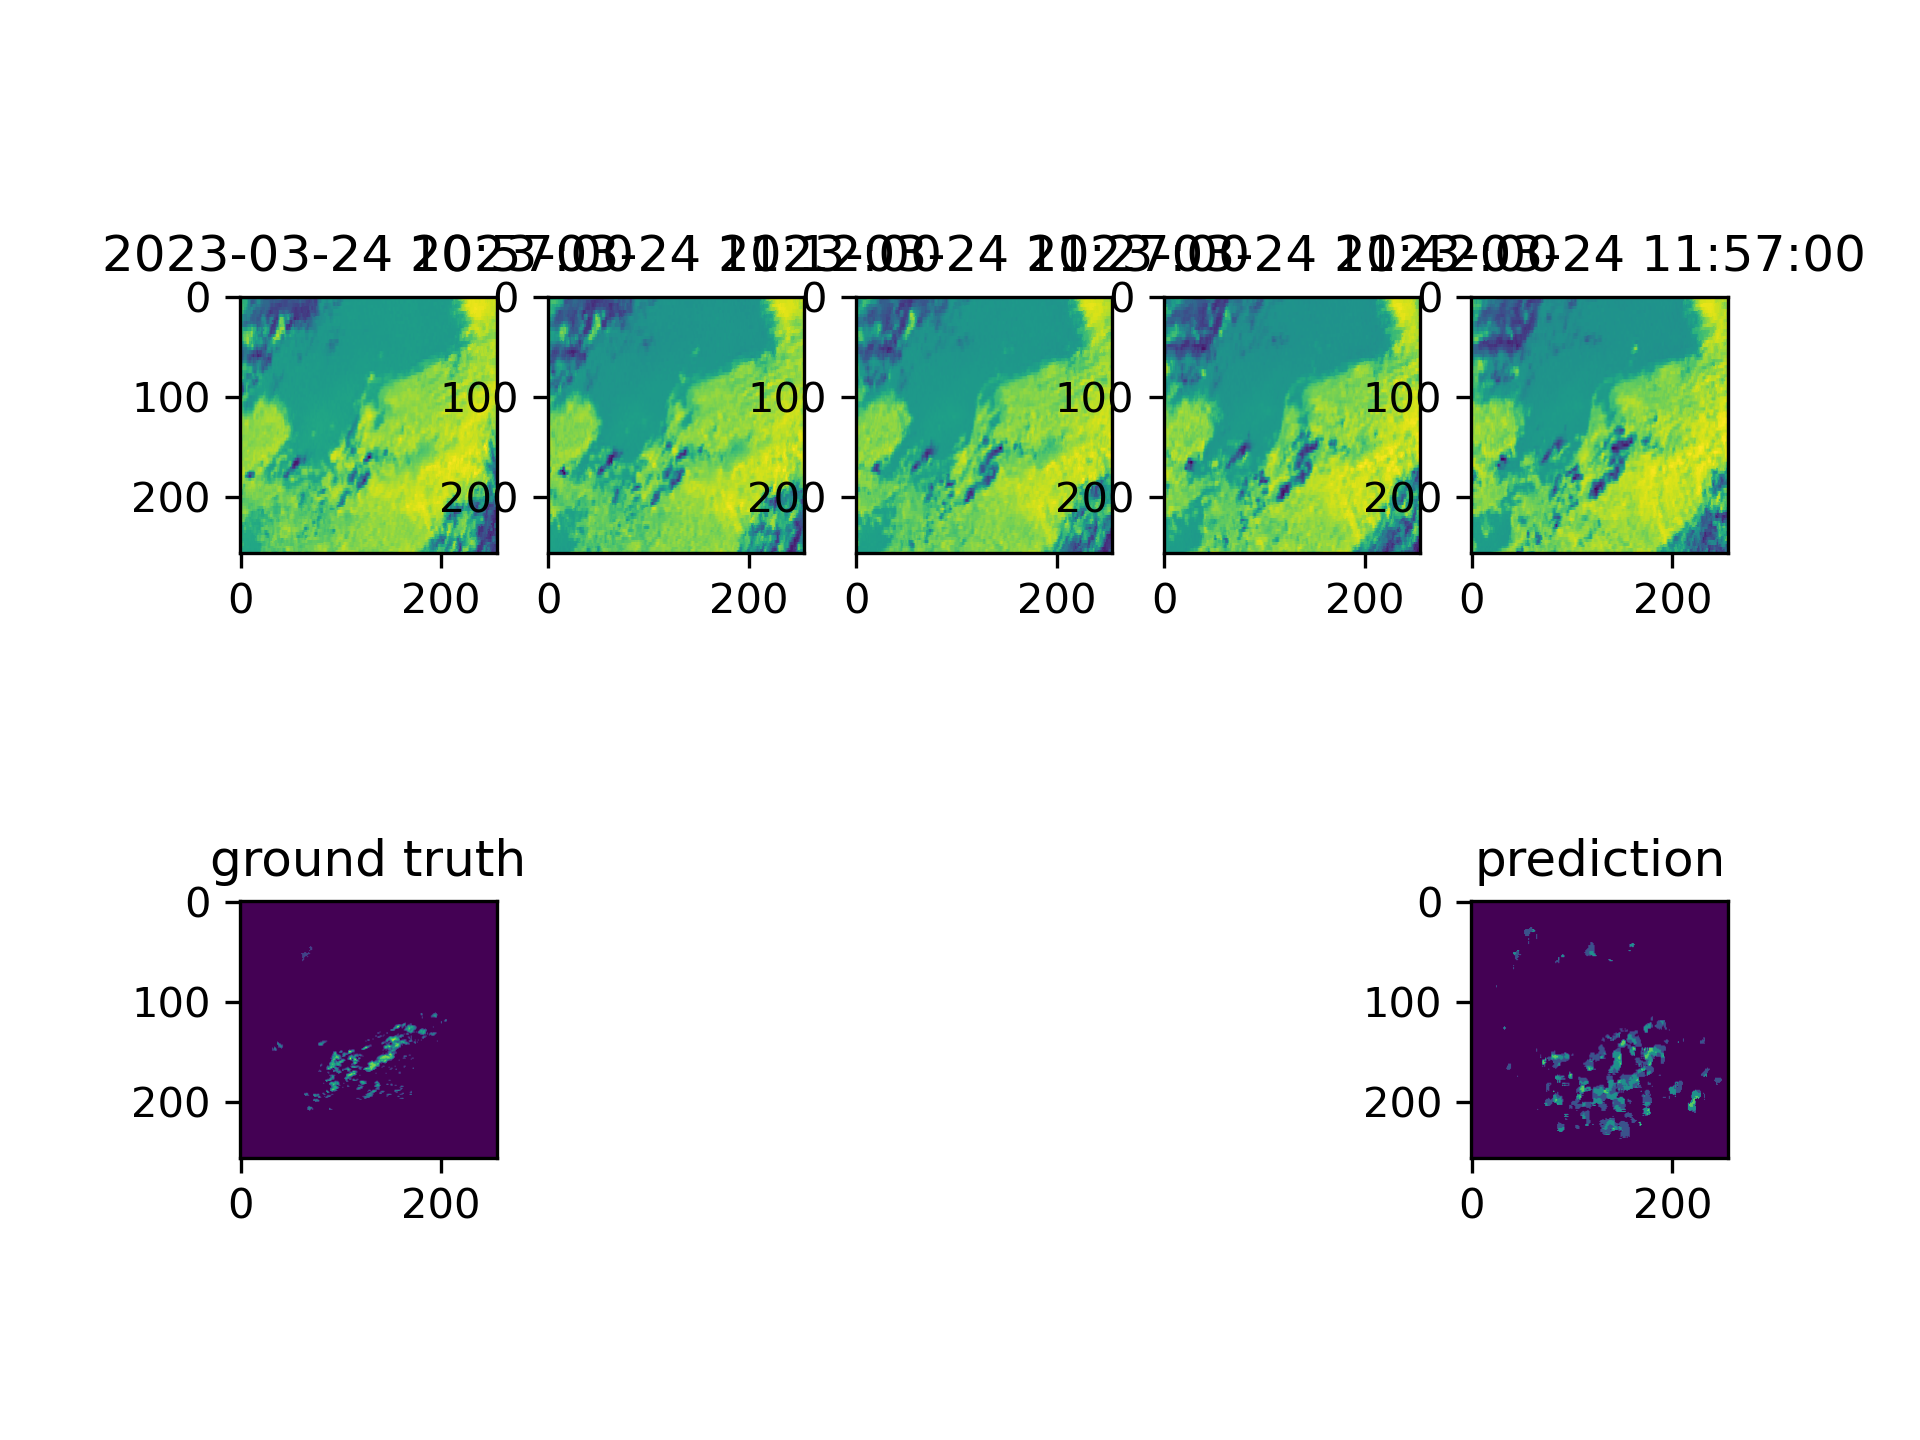
\includegraphics[width=225pt]{./images/experiment-0.png}
  \caption{Testset prediction with ConvLSTM model for 2023-03-24 12:02:00 UTC.}
  \Description{}
  \label{fig:convclass}
\end{figure*}

\begin{figure*}[hbp]
  \centering
  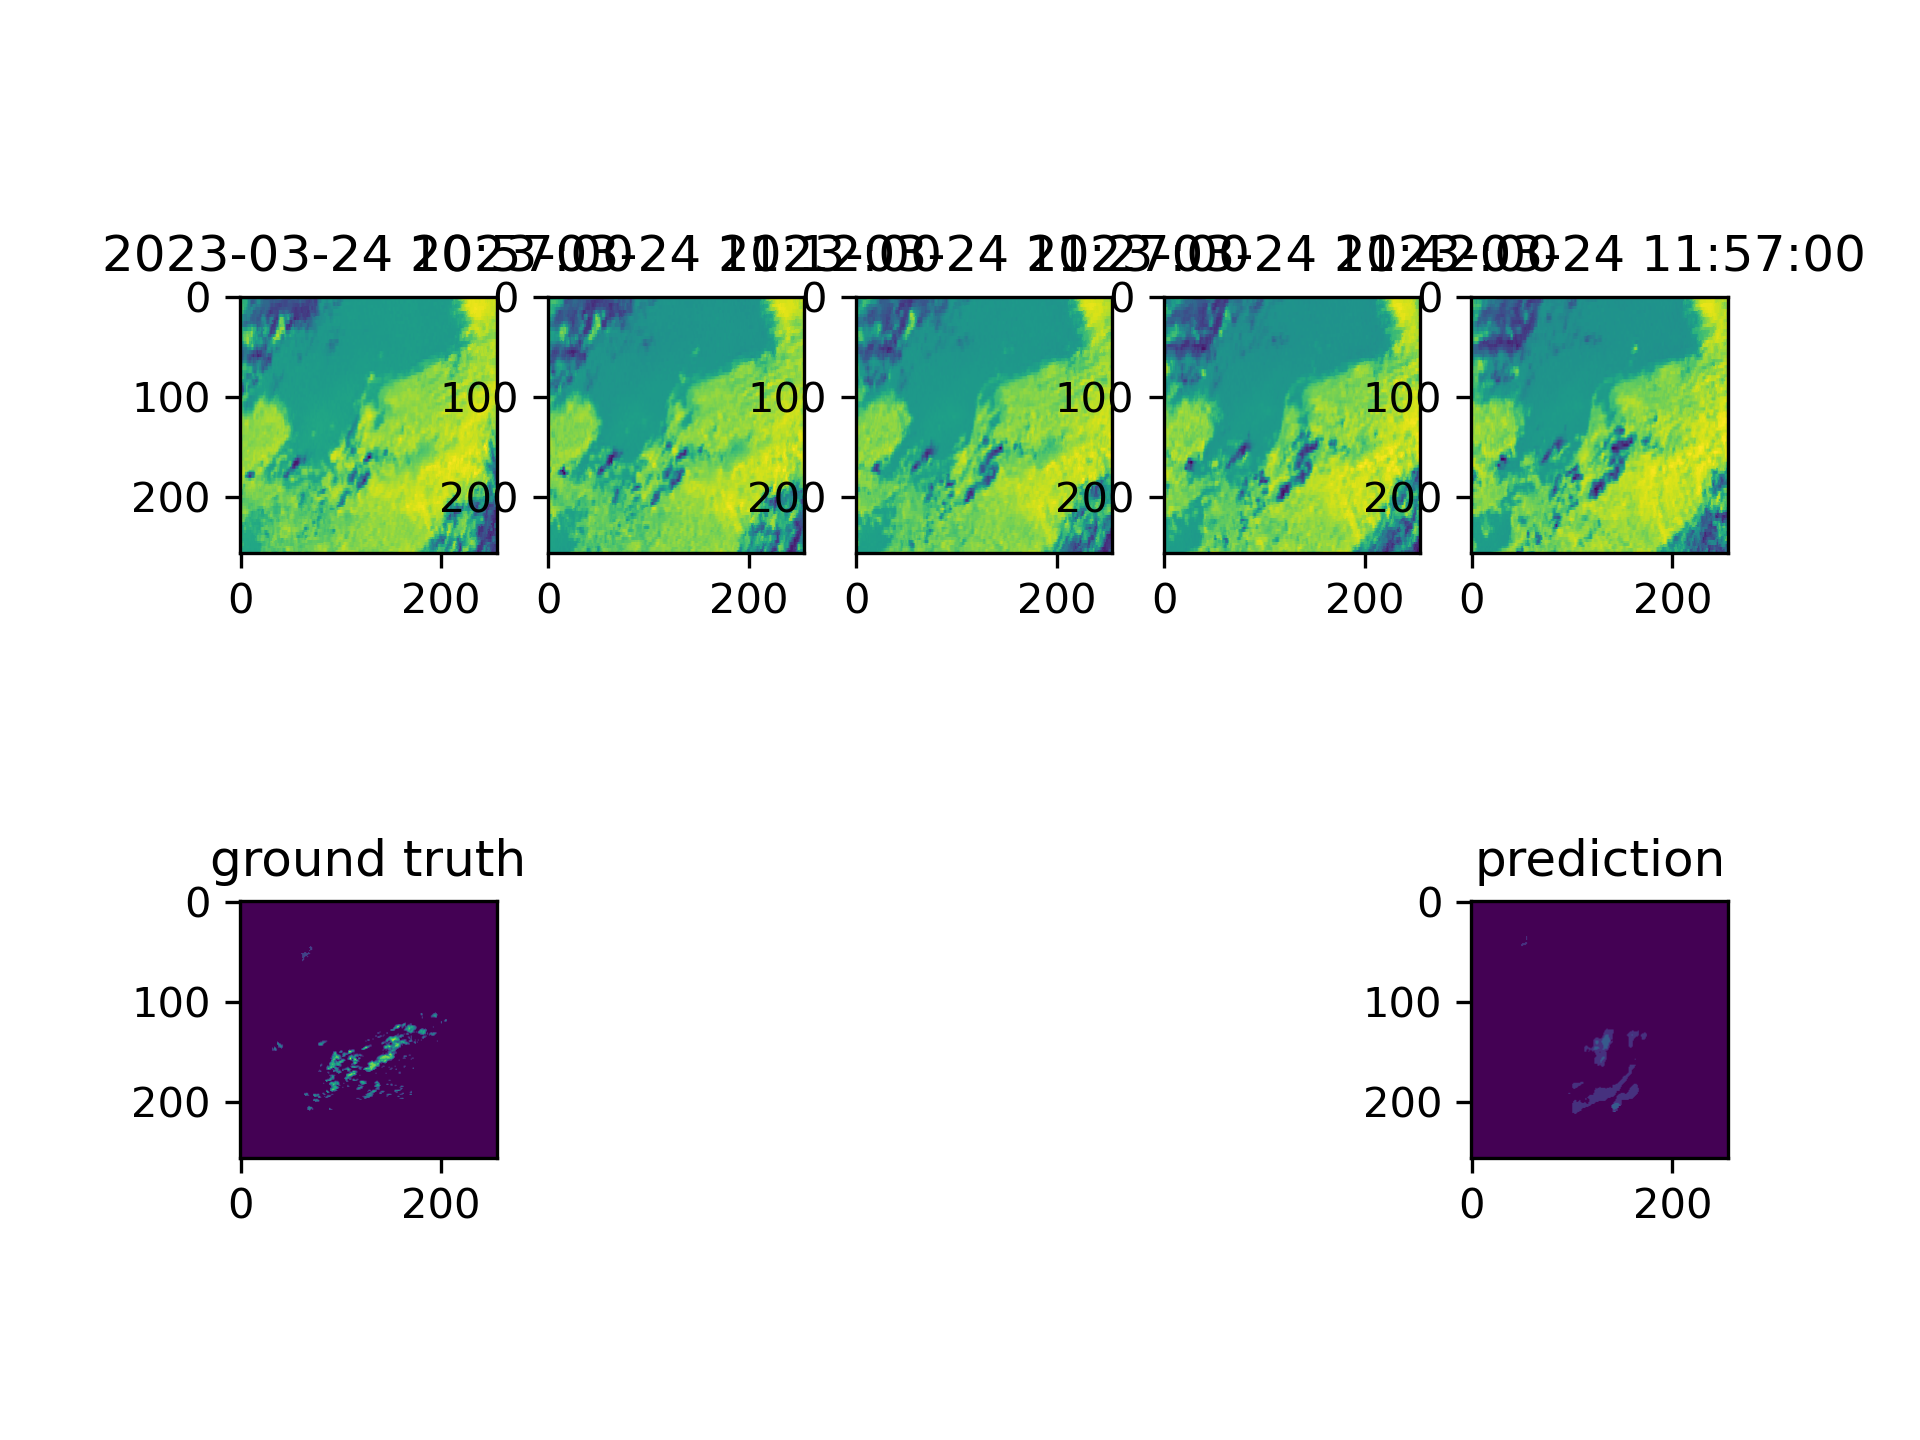
\includegraphics[width=225pt]{./images/experiment-0-unet.png}
  \caption{Testset prediction with U-Net model for 2023-03-24 12:02:00 UTC.}
  \Description{}
  \label{fig:unet}
\end{figure*}

\section{Future Work}
A core issue with this problem is data imbalance. There is data imbalance at two levels
first of all at the radar image level, frequencies for pixels containing rain are much lower than the opposite.
Secondly at the dataset level, the training, validation and test datasets contain different amounts of rain. Future work
could focus on created a curated dataset, that studies the amounts of rain in each partition and checks for sufficient rain events
in the training dataset.
Another avenue for future work could be working with alternative loss functions such as multi-class dice loss or focal loss.
Ensembling instead of training an end-to-end model could also be researched. For example by training a model to segment current available satellite images
to radar images and then train a different model with both the satellite images and segmented radar reflectivity images.
The problem also presents difficulties because the resolution of the satellite images is worse than the required output (3 vs 1 kilometer resolution).
This could be improved by using the high resolution visual channel of the satellite which has a 1km spatial resolution.

\section{Discussion}
A longer period is necessary to produce better results.

Model could be underfit, requiring more epochs and resources.

For U-Net the experimental setup is slightly different since we increased the available satellite timesteps from 5 to 8.
This is due to the fact that the encoder expects at least 8 in the depth dimension, to be able to encode the input patch.


A core issue with this problem is data imbalance. There is data imbalance at two levels.
First of all at the level of the datasets training, test and validation have different amounts of rain.
Optimally we would like to have a test dataset that has both stretches of time with large, and low amounts of precipitation.
As of now we have just cut off the datasets based on the available file count and the chosen split ratios.
Another source of data imbalance is the imbalance comes from the images. The radar images are most of the time presenting conditions with no rain.
When there is rain present on the images it is rare that this surpasses 50\% of the image. This makes it difficult to produce suitable models because
the model is biased towards predicting no rain. We have used known methods for imbalanced datasets such as adding class weights to 
the loss function. Other methods such as focal loss exist, which could be investigated in further research.

The problem also presents difficulties because the resolution of the satellite images is worse than the required output.
This could be improved with the high resolution visual channel of the satellite which has a 1km spatial  resolution.

radar and satellite pixels are not perfectly aligned grids.
radar has more spatial resolution 1x1 km while satellite has 3x3 km at the
sub satellite point. At the edge each pixel covers 12km area.

\begin{figure}
    \centering
    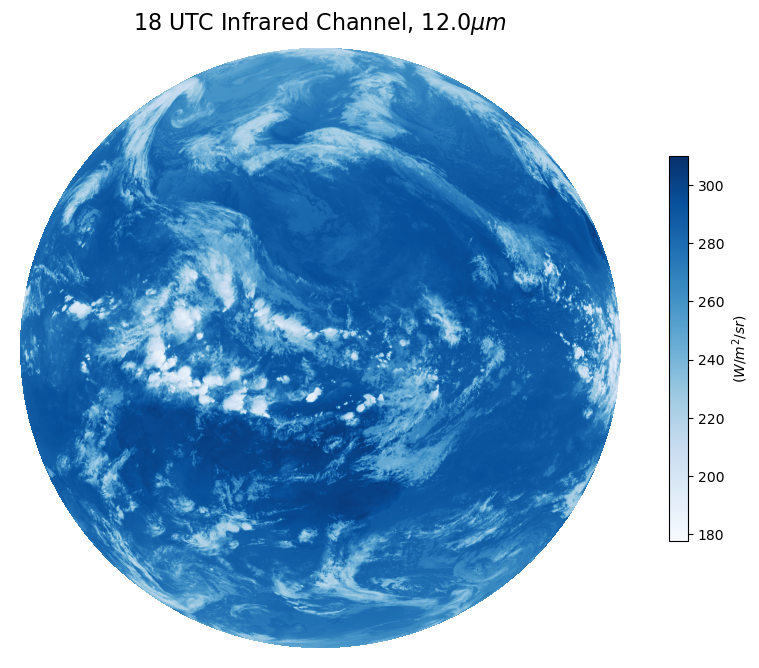
\includegraphics[width=225pt]{./images/infrared.png}
    \caption{Satellite Image: Infrared Channel 18UTC $12.0\mu m$}
    \Description{Satellite Image of the earth}
    \label{fig:infra}
\end{figure}


\section{Conclusions}
In this paper we investigate whether it is possible to create
a model to predict precipitation with only sequences radar inputs.
We found key aspects that need to be addressed in order to build a well performing model.
These aspects are a model architecture that supports a time dimension such as RNNs or 3D Unet.
Then a method to work with imbalanced data, weighting the loss function.
The methods that can be used to create this model, are shown to be ConvLSTM and 3D Unet based models 
although other methods may be valid but we have not tested them.
.
The model appears to not be very effective from a visual inspection 

\begin{acks}
I would like to thank my supervisor from Elena Mocanu, for her help. Furthermore I would like to thank I would like to thank Dina Lazorkeno for proofreading my thesis.
\end{acks}

\bibliographystyle{ACM-Reference-Format}
\bibliography{ref}

\newpage
\appendix
\large{Appenices}

\section{Images}

\begin{figure*}[hbp]
  \centering
  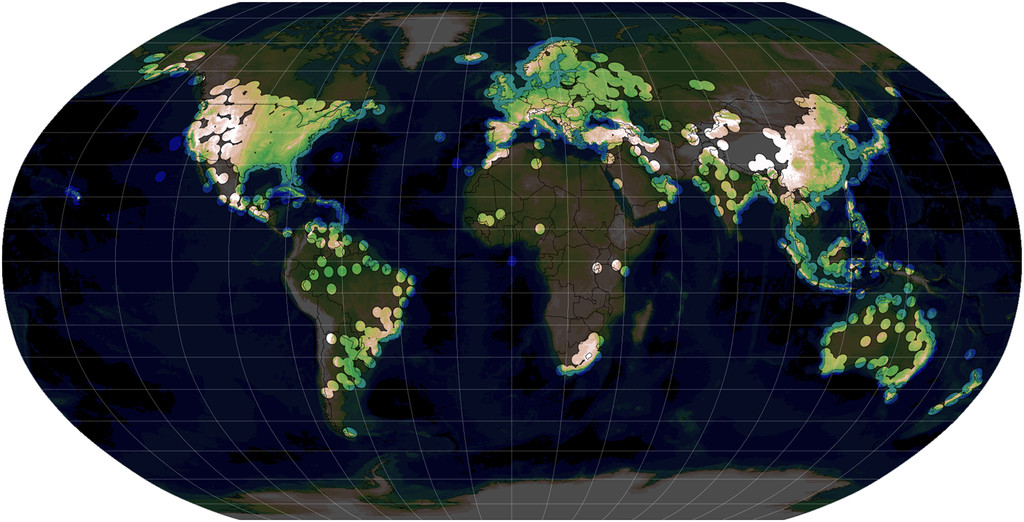
\includegraphics[width=400pt]{./images/full-bams-d-18-0166.1-f1.jpg}
  \caption{Worldwide availability of radar data. Notably Oceans; the African and South American continents lack good coverage. \cite{AnOverviewofUsingWeatherRadarforClimatologicalStudiesSuccessesChallengesandPotential}}
  \Description{}
  \label{fig:radar-availability}
\end{figure*}

\begin{figure}[hbp]
  \centering
  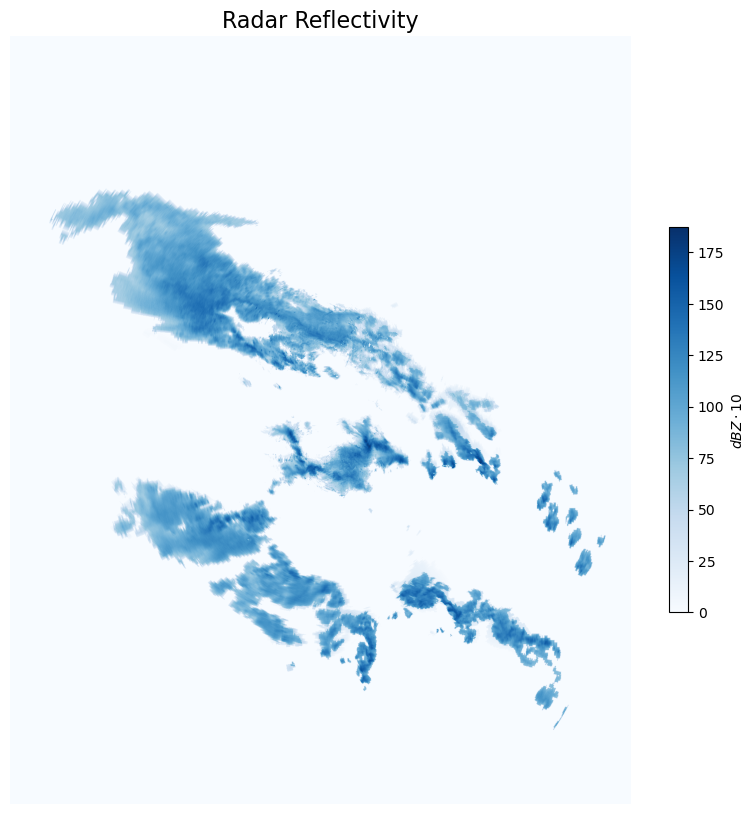
\includegraphics[width=225pt]{./images/radar_reflectivity.png}
  \caption{Radar Reflectivity}
  \Description{}
  \label{fig:reflect}
\end{figure}

\begin{figure}[hbp]
  \centering
  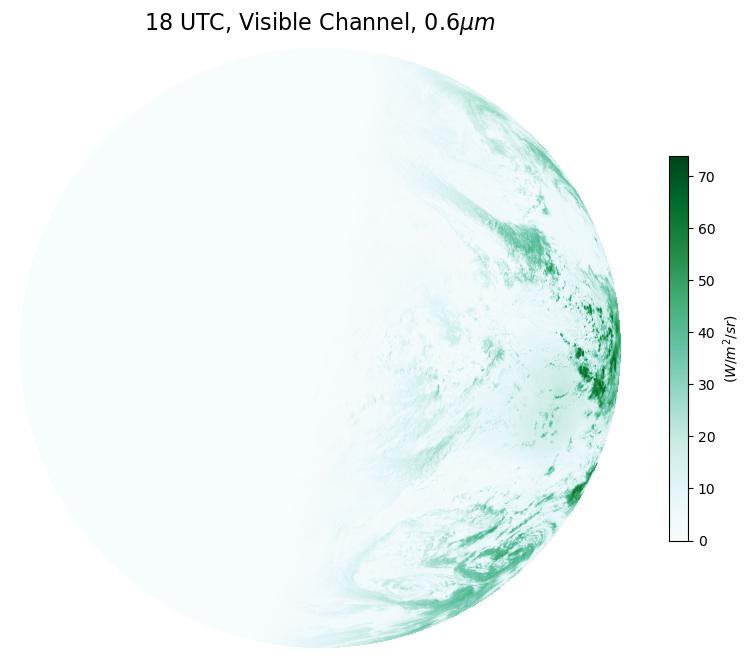
\includegraphics[width=225pt]{./images/vis_006.png}
  \caption{Satellite Image: Visible Channel 18UTC $0.6\mu m$}
  \Description{}
  \label{fig:vis}
\end{figure}

\begin{figure}[hbp]
  \centering
  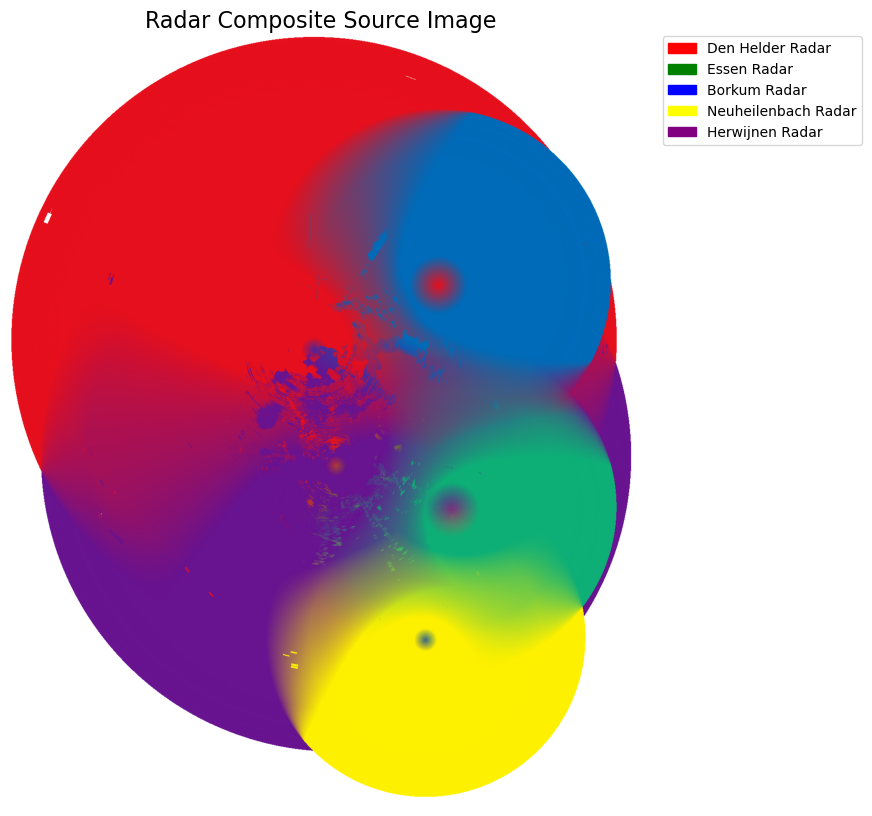
\includegraphics[width=225pt]{./images/radar_source.png}
  \caption{Used Composite Radar Image Source. Colors mapping to 5 different radars: Den Helder, Essen, Borkum, Neuheilenbach and Herwijnen.}
  \Description{}
  \label{fig:radsource}
\end{figure}

\begin{figure}[hbp]
  \centering
  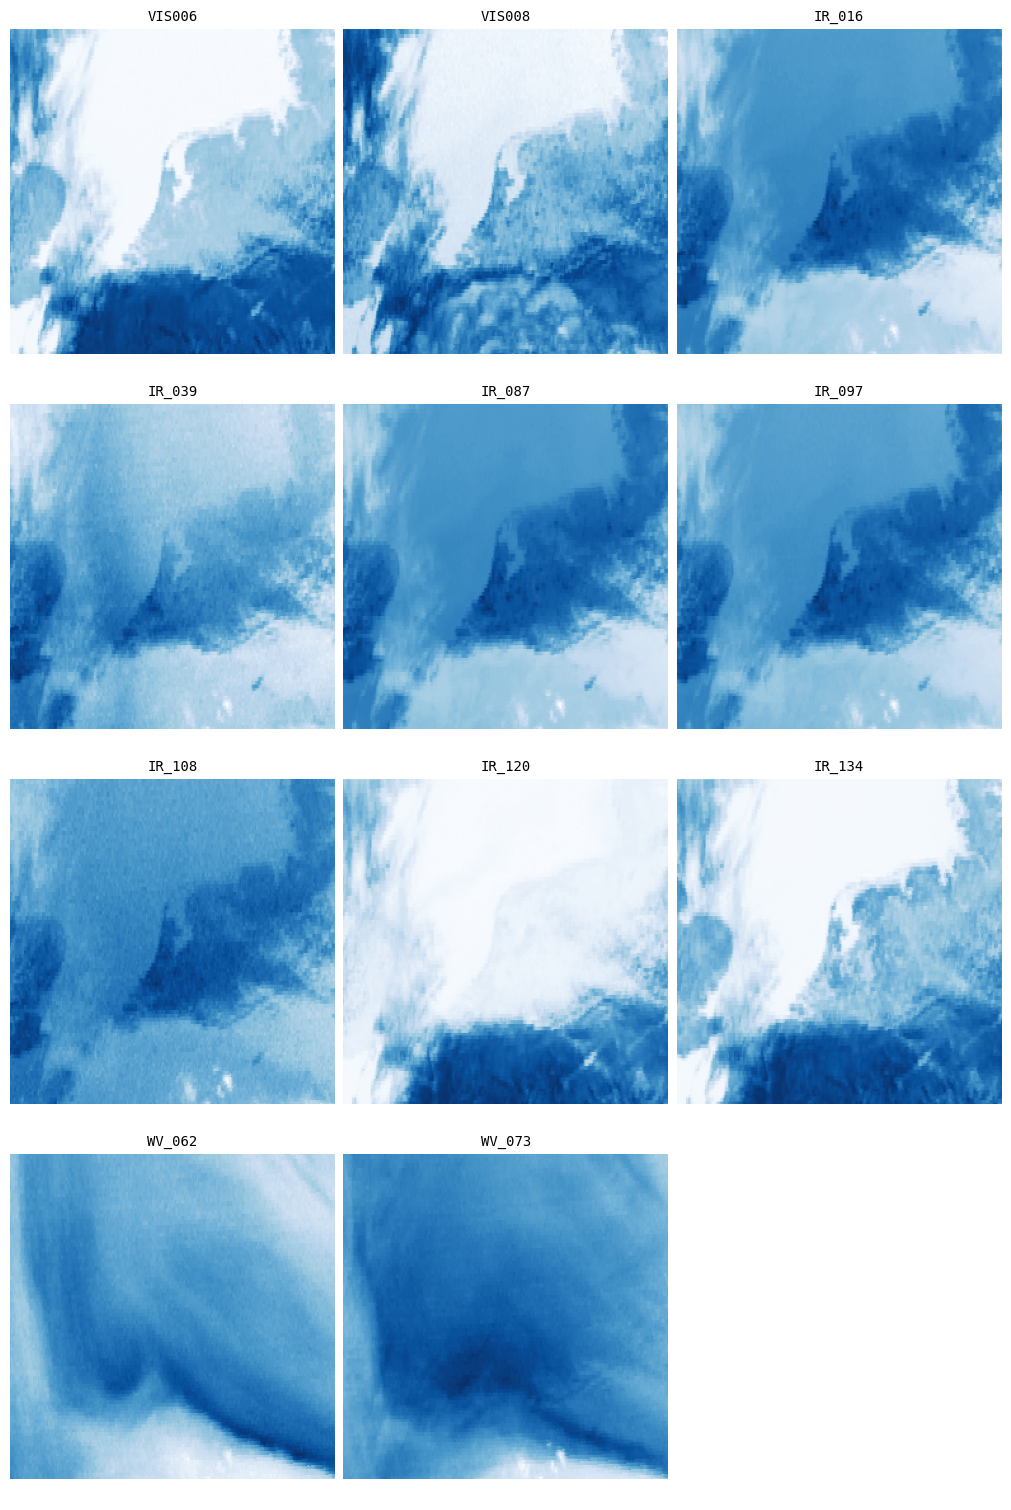
\includegraphics[width=250pt]{./images/single_satellite.png}
  \caption{Preprocessed Satellite Image}
  \Description{}
  \label{fig:satchannels}
\end{figure}

\begin{figure}[hbp]
  \centering
  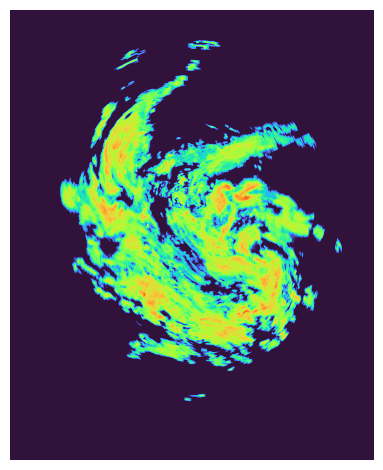
\includegraphics[width=200pt]{./images/radar_image.png}
  \caption{Preprocessed Satellite Image}
  \Description{}
  \label{fig:radar-pre}
\end{figure}

\begin{figure}[hbp]
  \centering
  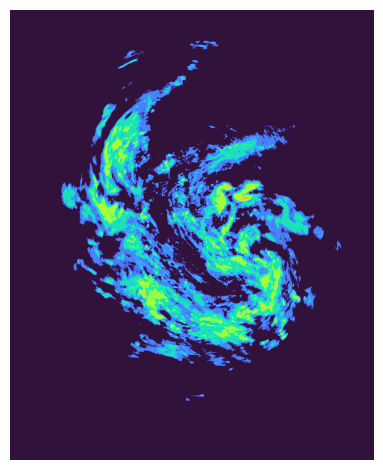
\includegraphics[width=200pt]{./images/radar_binned.png}
  \caption{Preprocessed Satellite Image}
  \Description{}
  \label{fig:radar-bin}
\end{figure}

\begin{figure*}[hbp]
  \centering
  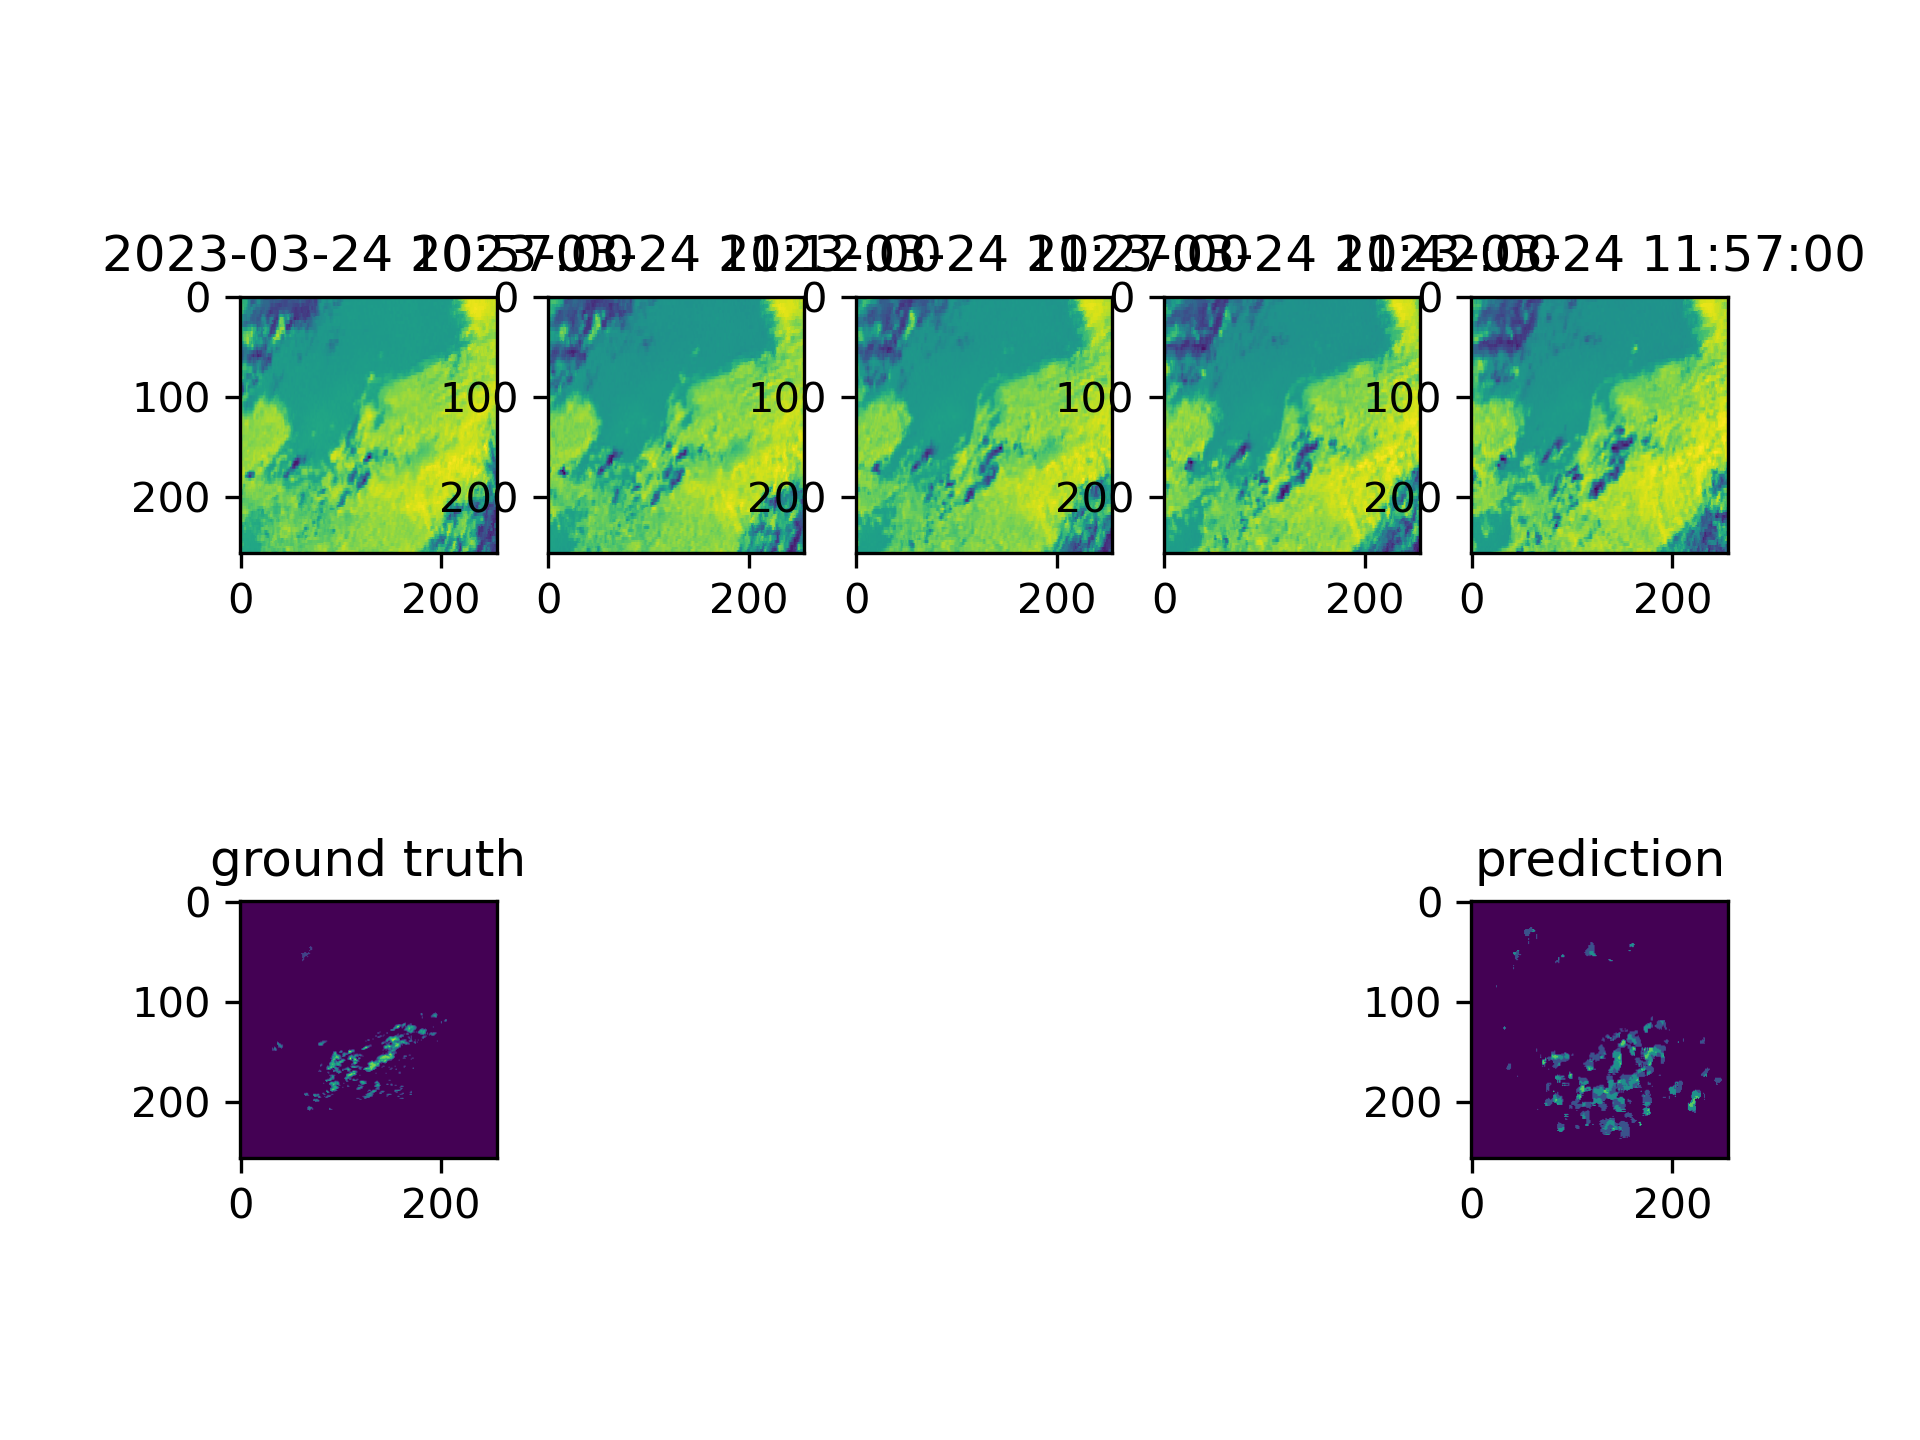
\includegraphics[width=500pt]{./images/experiment-0.png}
  \caption{Testset prediction with ConvLSTM model for 2023-03-24 12:02:00 UTC.}
  \Description{}
  \label{fig:convclass}
\end{figure*}

\begin{figure*}[hbp]
  \centering
  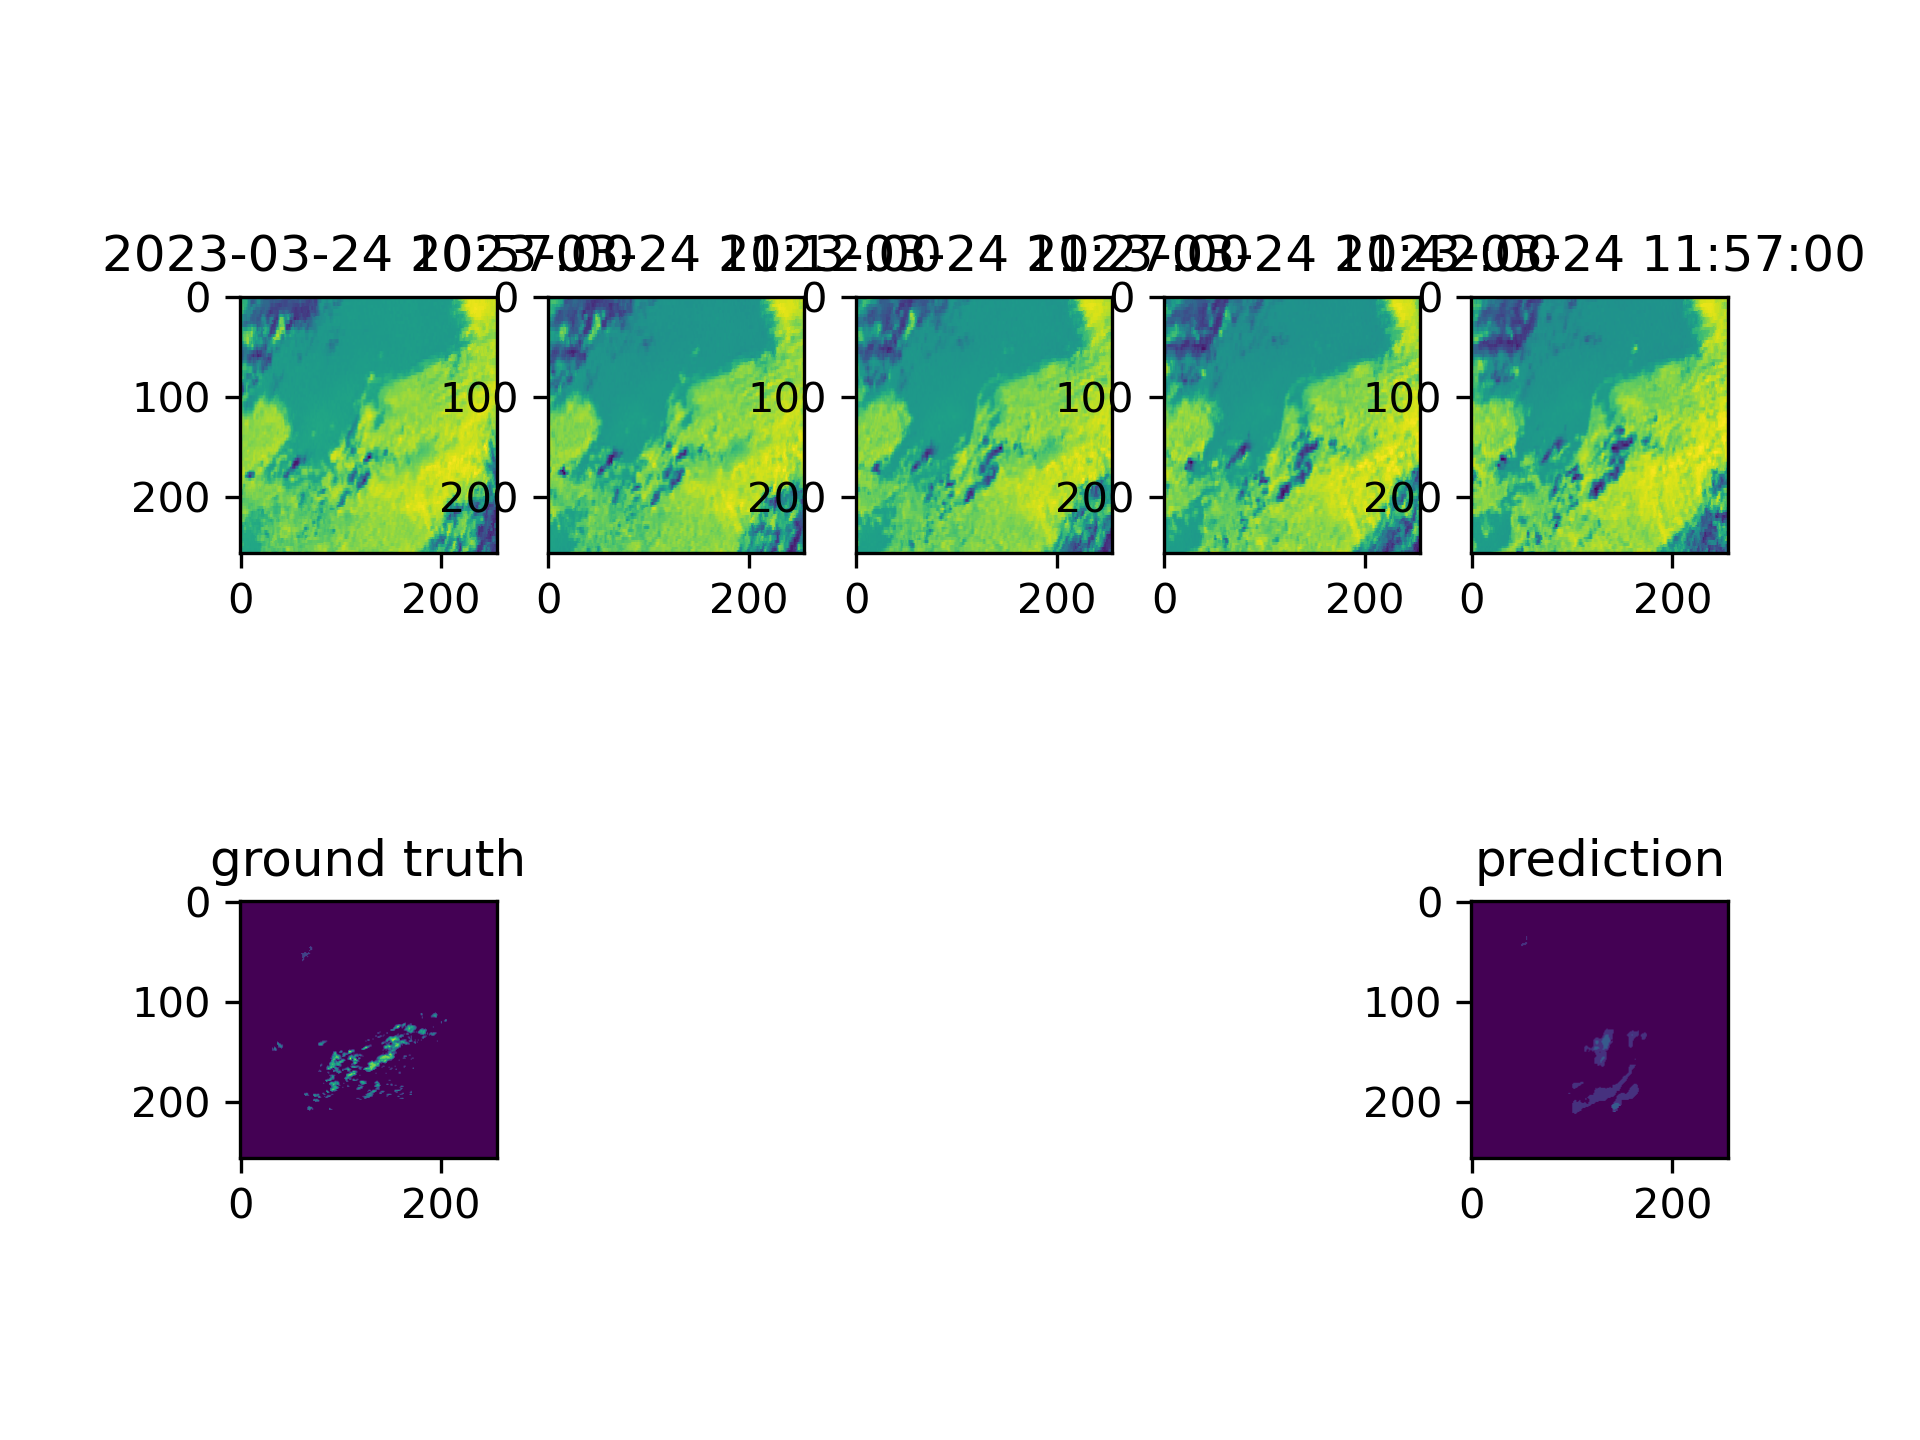
\includegraphics[width=500pt]{./images/experiment-0-unet.png}
  \caption{Testset prediction with U-Net model for 2023-03-24 12:02:00 UTC.}
  \Description{}
  \label{fig:unet}
\end{figure*}
\begin{figure*}[hbp]
  \centering
  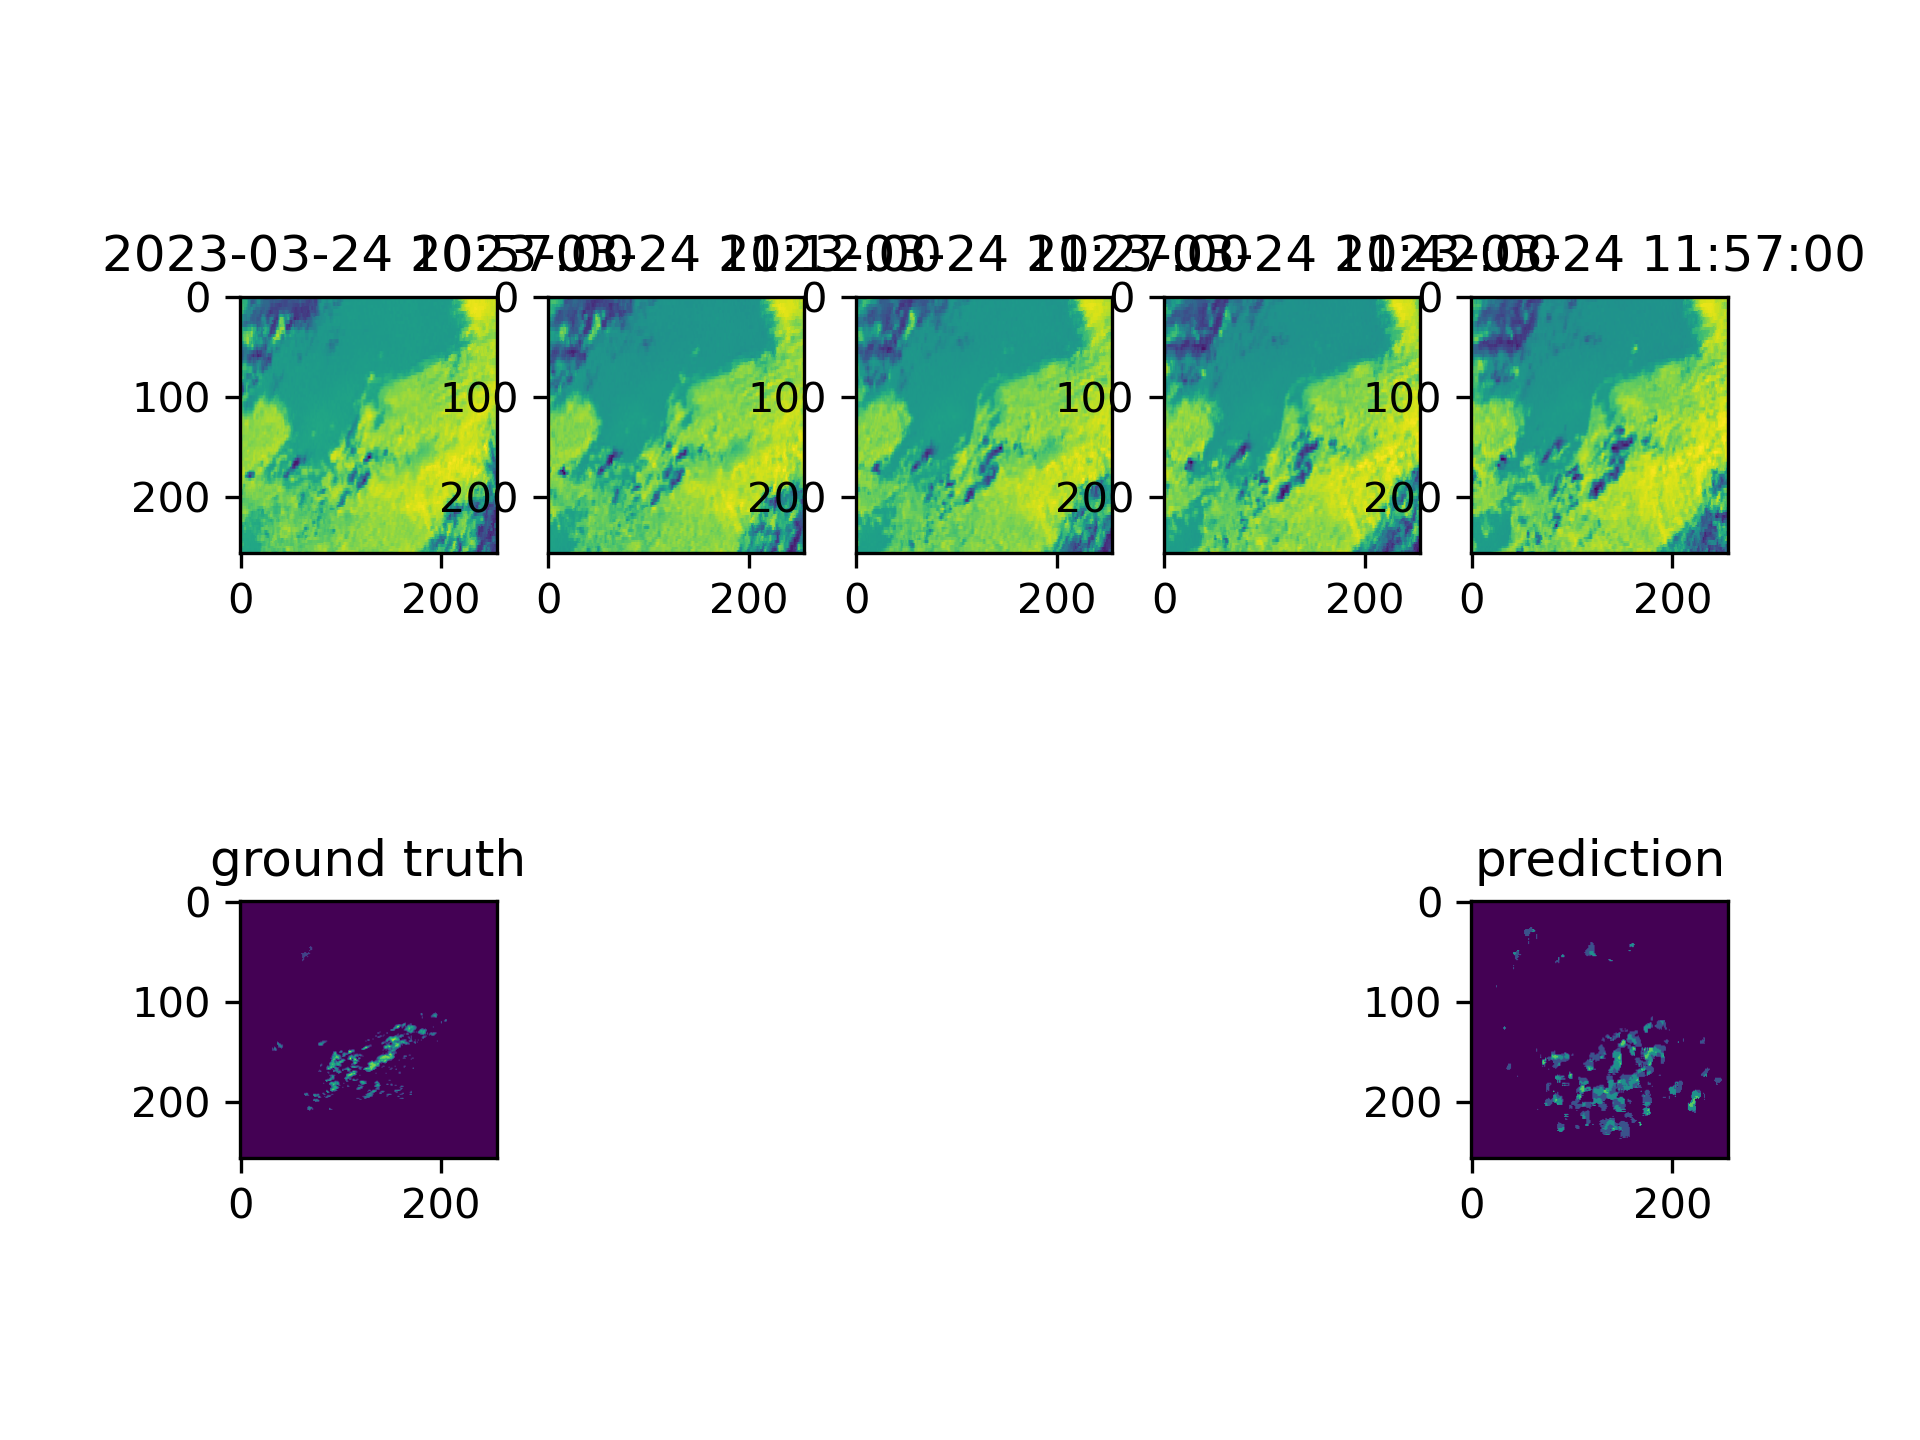
\includegraphics[width=500pt]{./images/experiment-0.png}
  \caption{Testset prediction with ConvLSTM model for 2023-03-24 12:02:00 UTC.}
  \Description{}
  \label{fig:convclass}
\end{figure*}

\begin{figure*}[hbp]
  \centering
  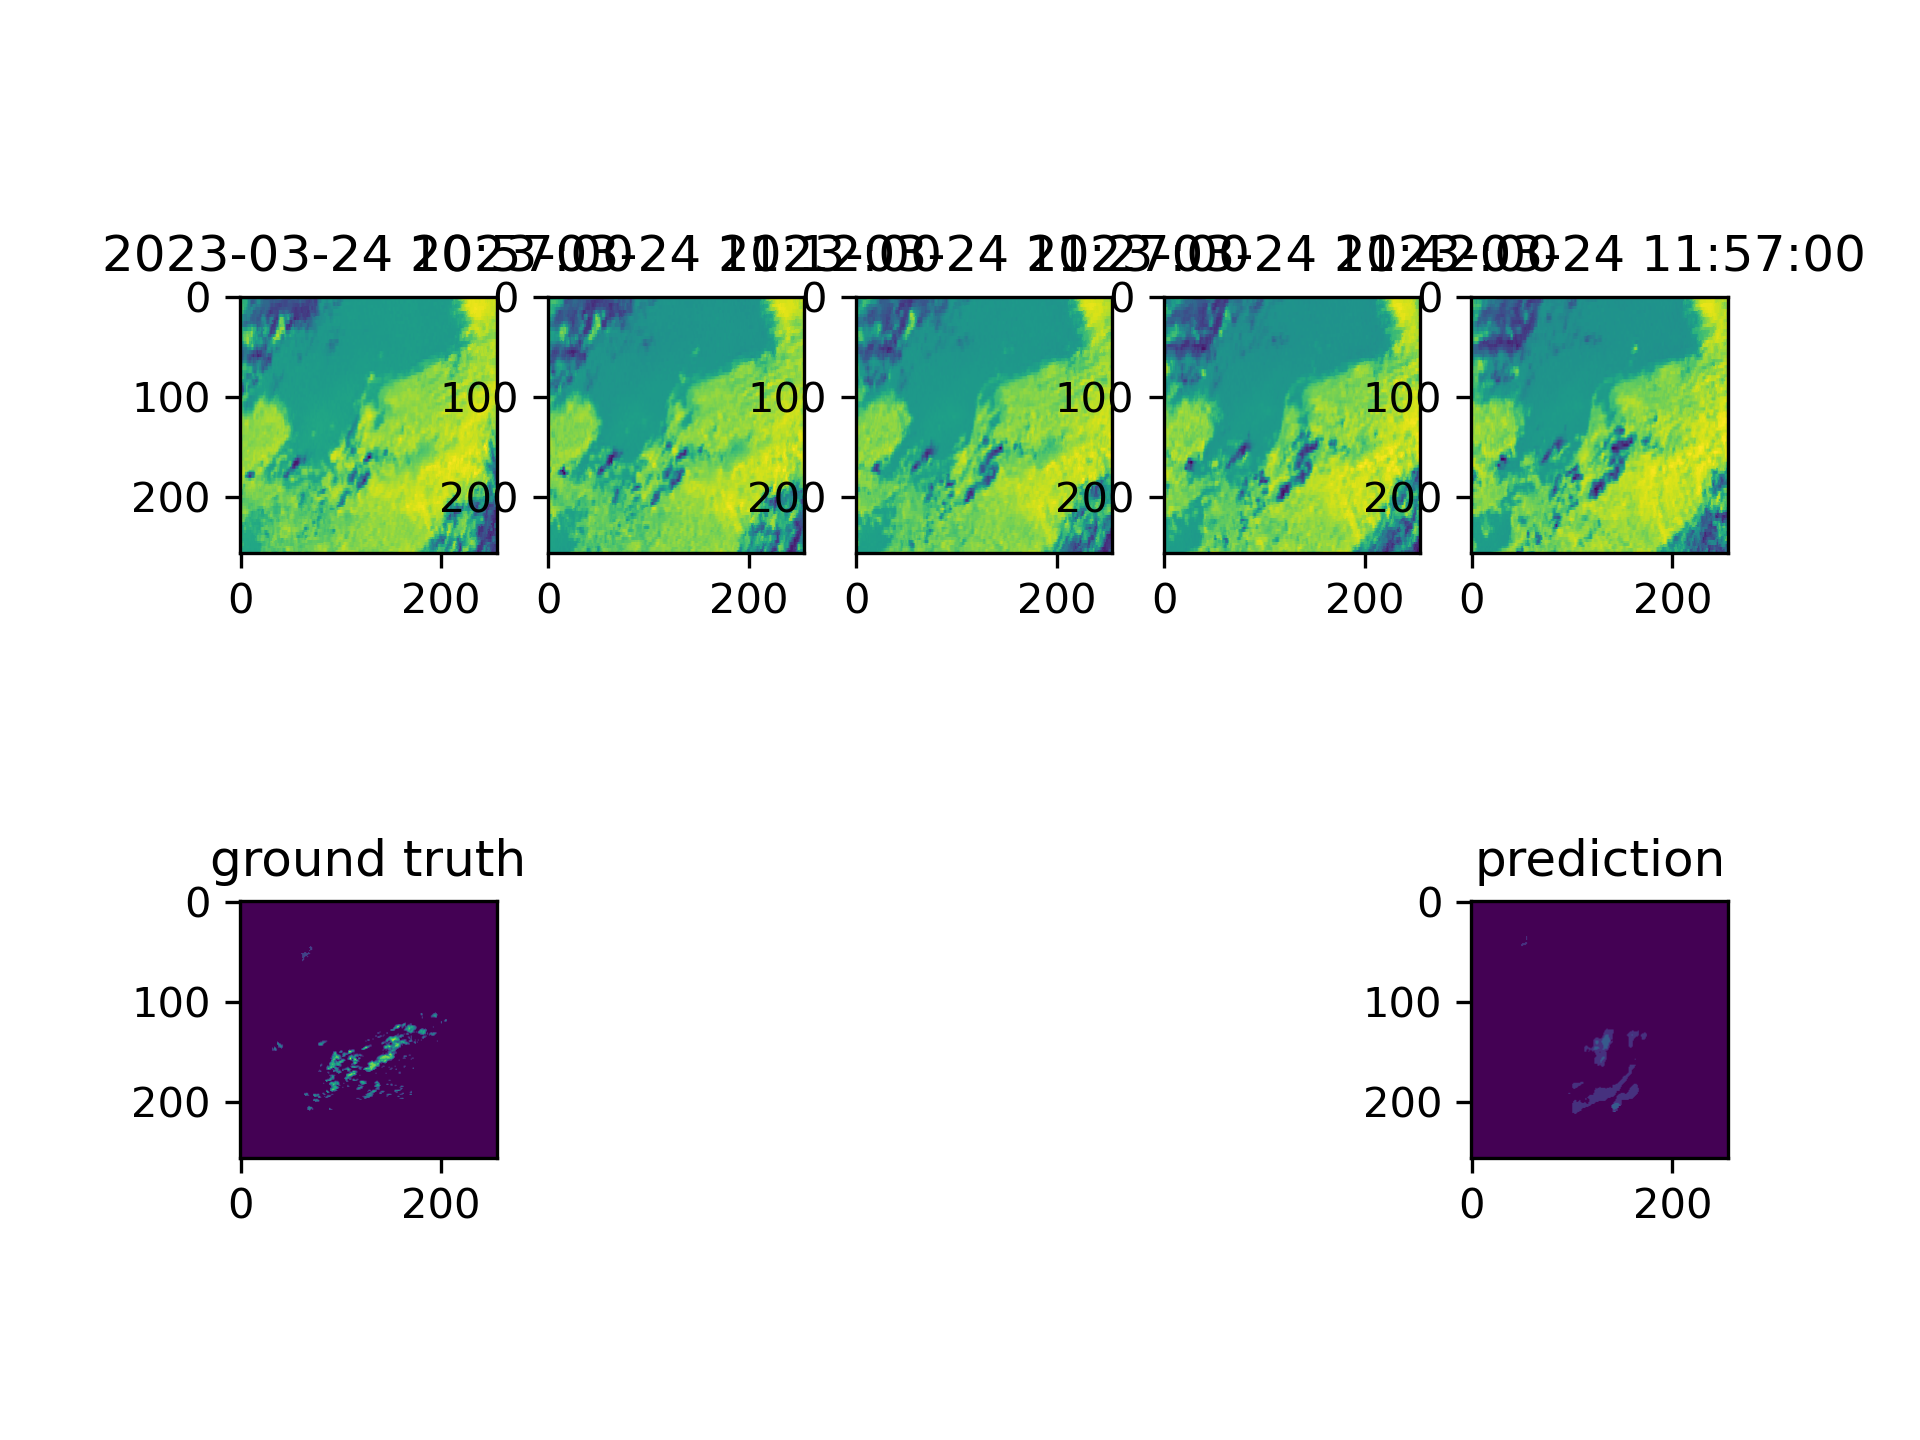
\includegraphics[width=500pt]{./images/experiment-0-unet.png}
  \caption{Testset prediction with U-Net model for 2023-03-24 12:02:00 UTC.}
  \Description{}
  \label{fig:unet}
\end{figure*}

\begin{figure*}[hbp]
  \centering
  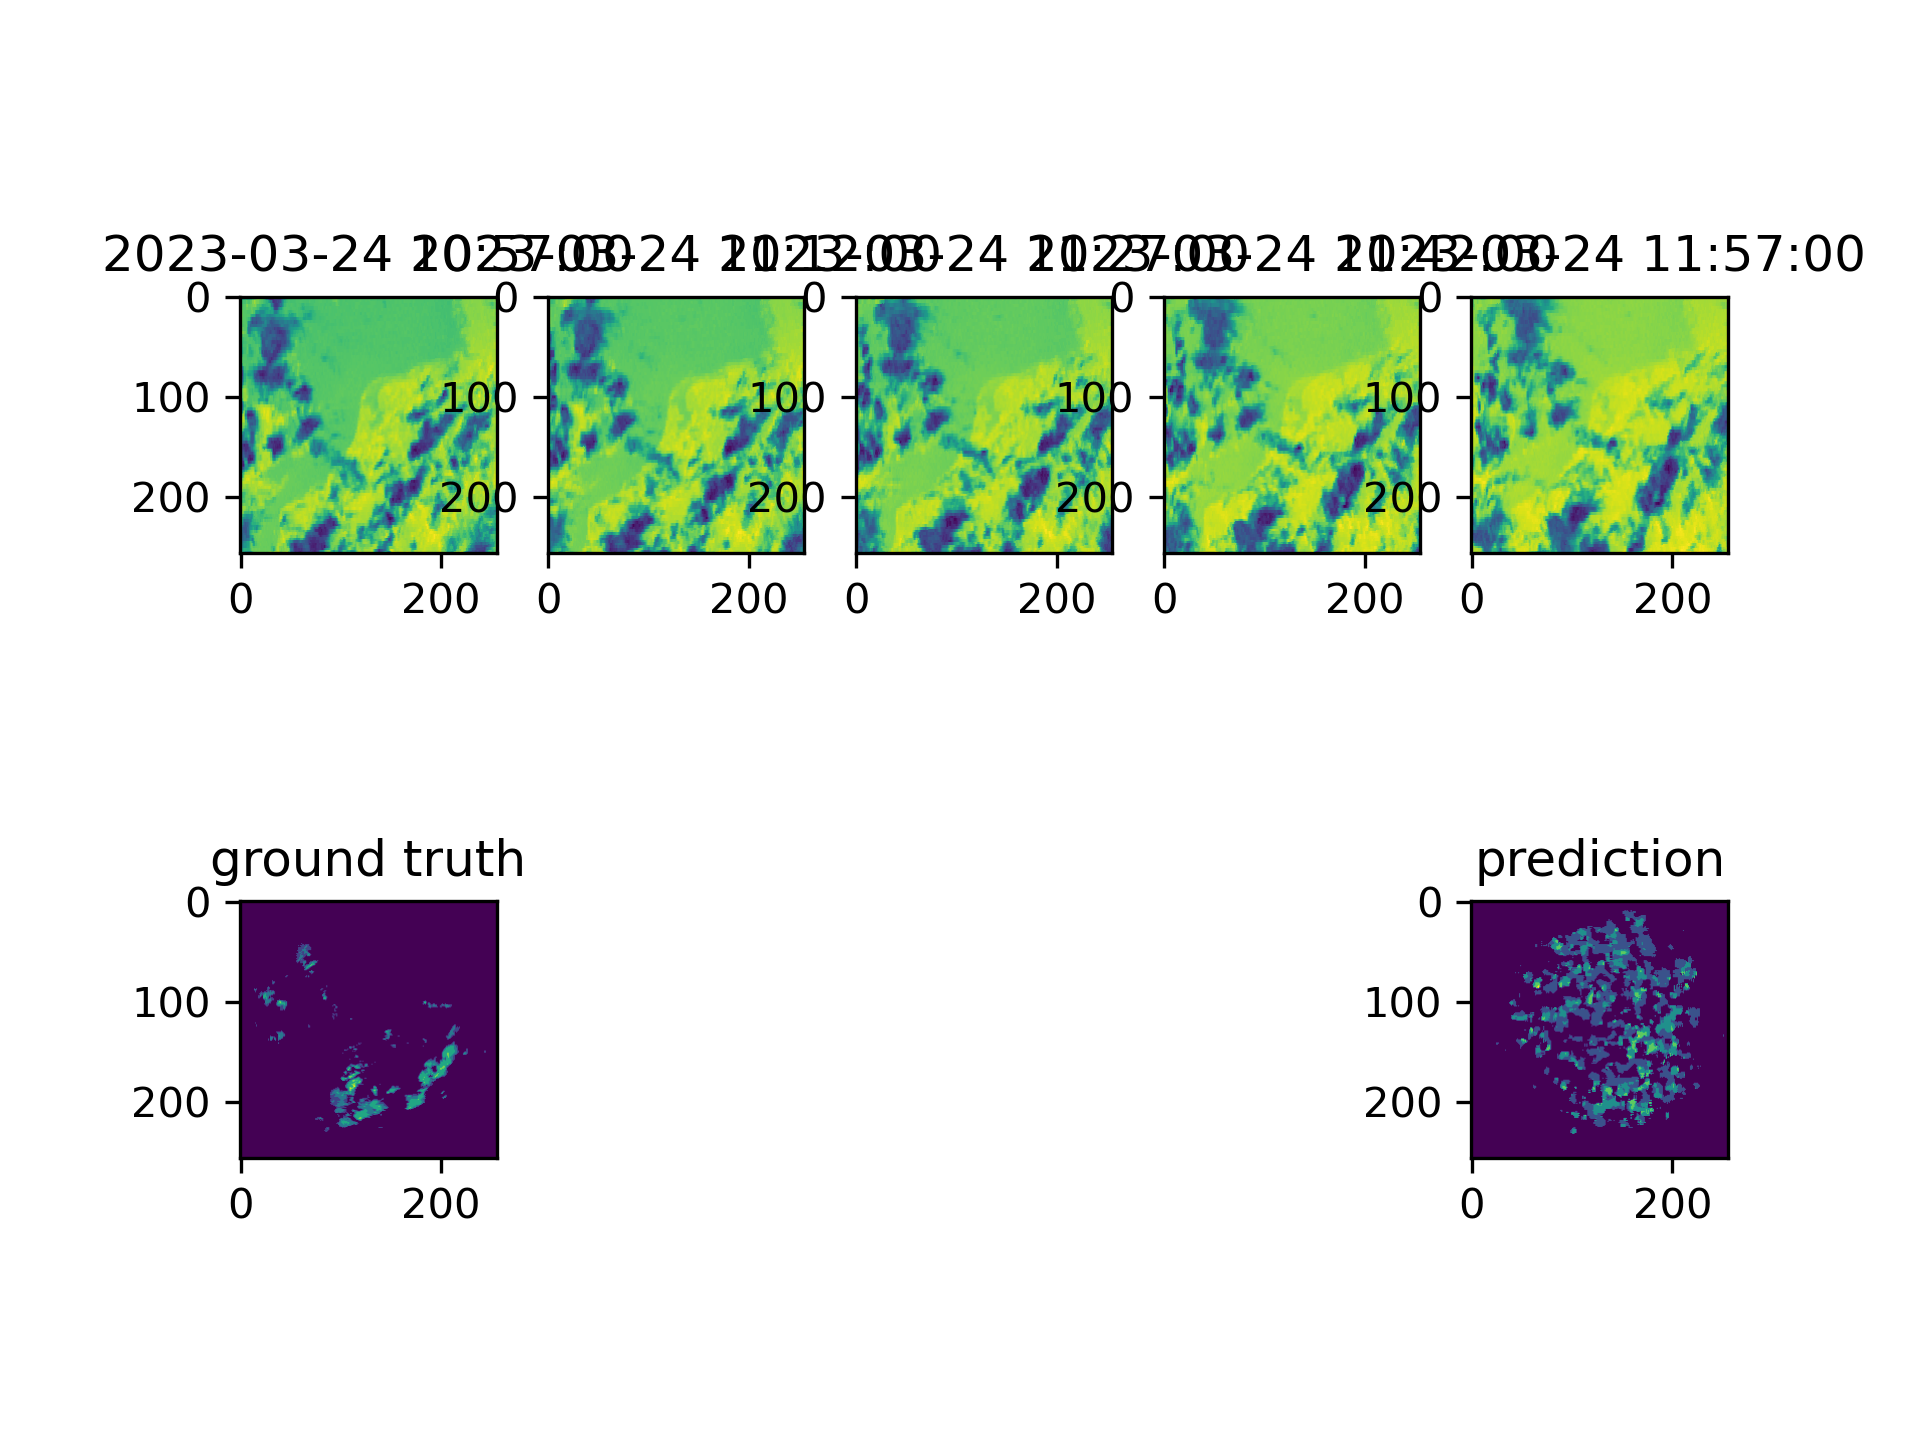
\includegraphics[width=400pt]{./images/experiment-19.png}
  \caption{Testset Prediction ConvLSTM}
  \Description{}
  \label{fig:experiment-19}
\end{figure*}

\begin{figure*}[hbp]
  \centering
  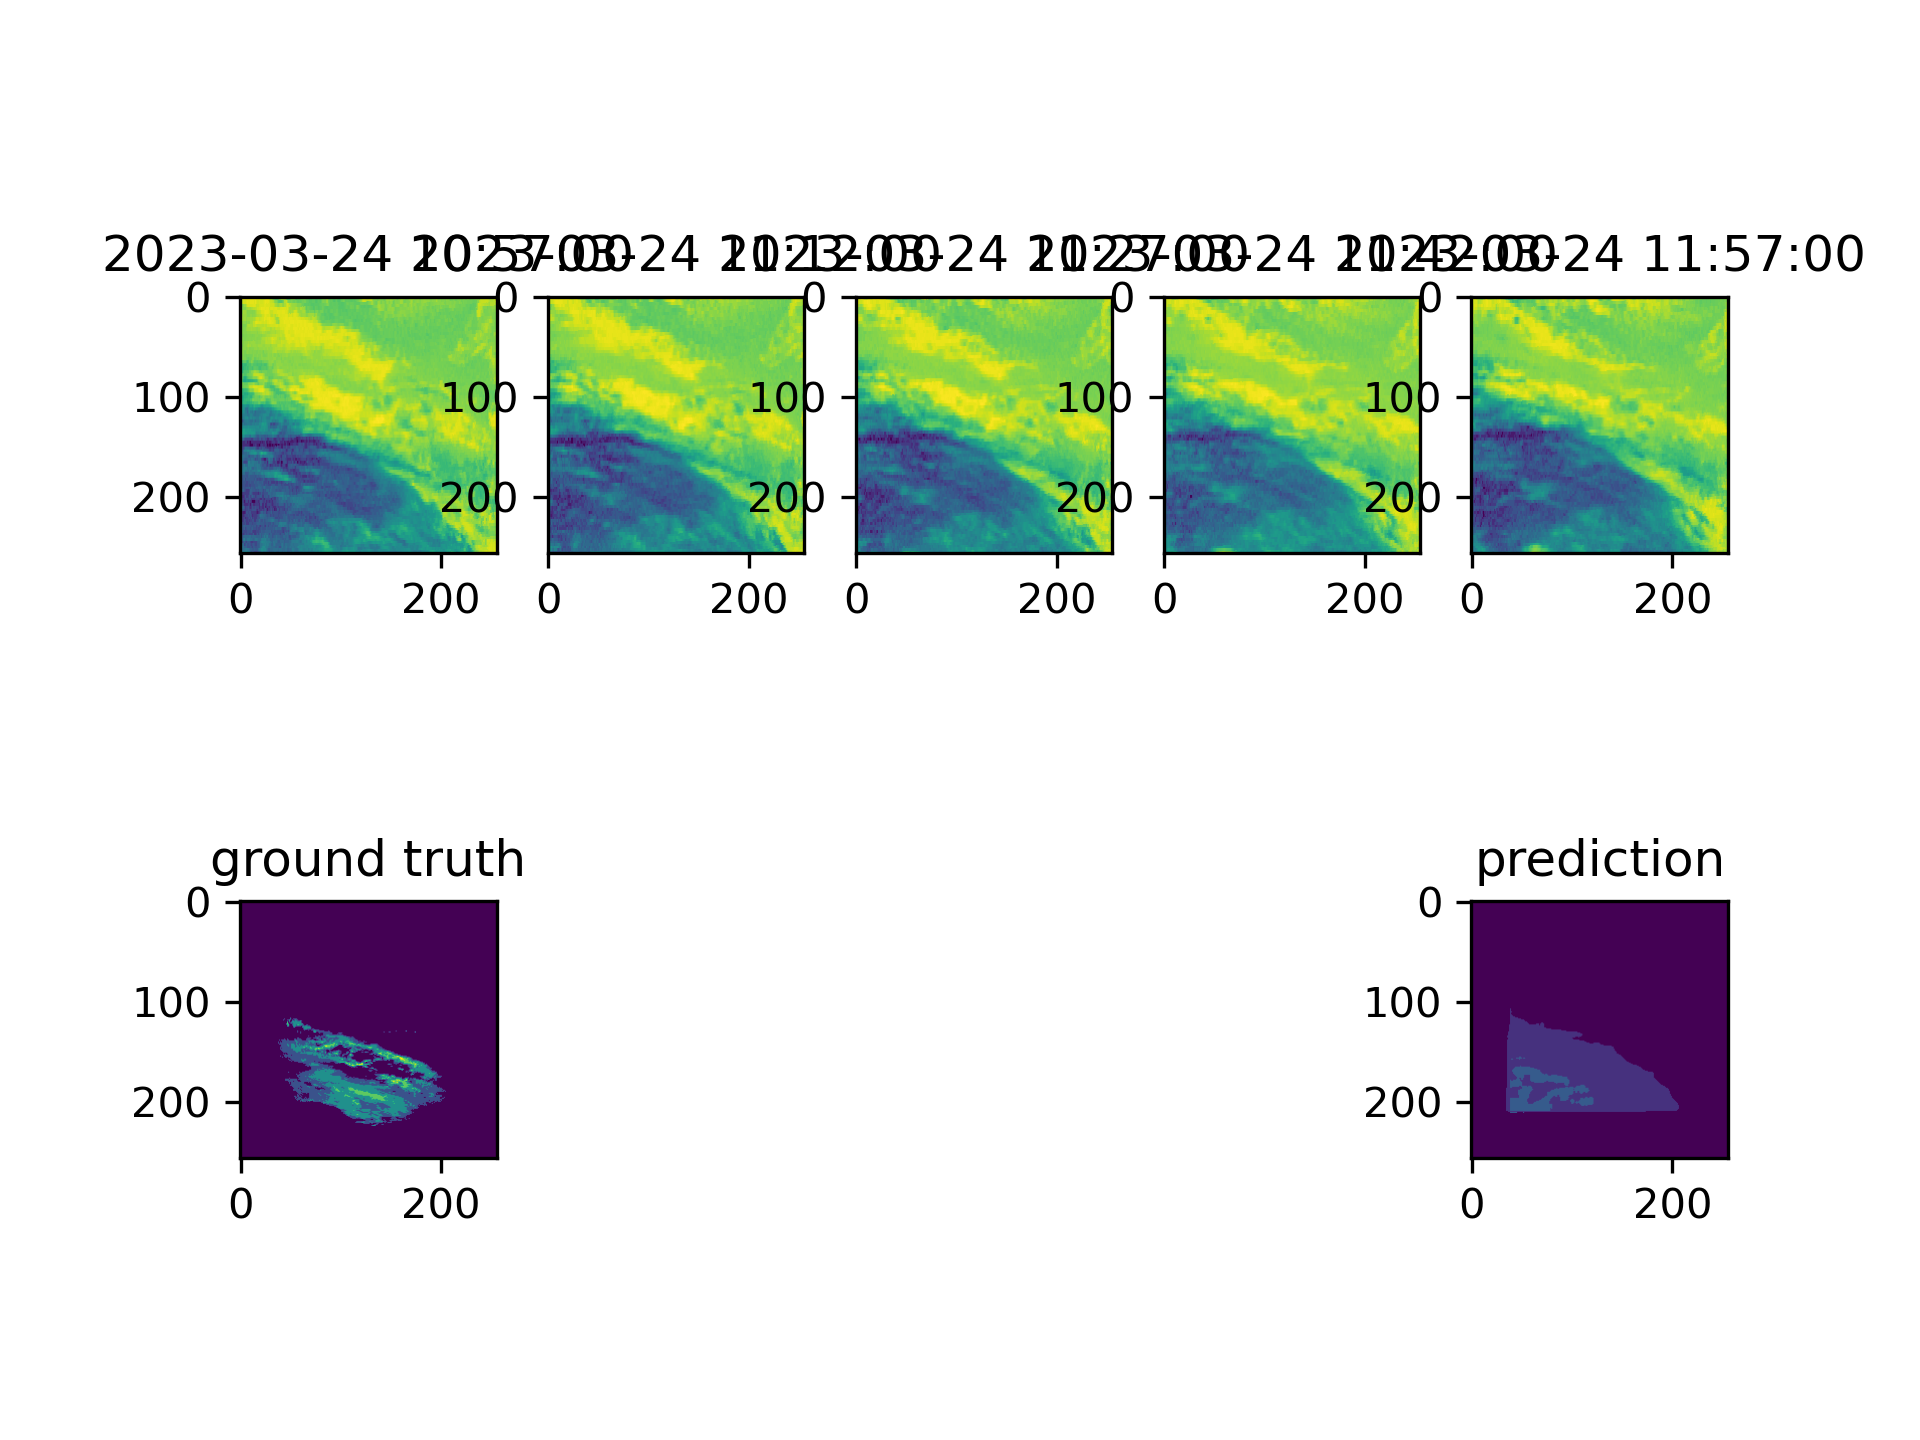
\includegraphics[width=400pt]{./images/experiment-160.png}
  \caption{Testset Prediction 3D U-Net}
  \Description{}
  \label{fig:experiment-160}
\end{figure*}

\newpage
\section{Tables}

\begin{table}[]
  \caption{Available Classes for Classification Models. Based on intervals of 10 dBZ in a interval between 0 and 60}
  \begin{tabular}{@{}ll@{}}
  \toprule
  Class & dBZ range   \\ \midrule
  0     & $(-\infty, 0]$ \\
  1     & $(0, 10]$  \\
  2     & $(10, 20]$  \\
  3     & $(20, 30]$  \\
  4     & $(30, 40]$  \\
  5     & $(40, 50]$  \\
  6     & $(50, 60]$  \\
  7     & $(60, +\infty)$  \\ \bottomrule
  \end{tabular}
\end{table}

\begin{table}[hbp]
  \caption{Available Satellite Channels.}
  \begin{tabular}{@{}lll@{}}
  \toprule
  Channel & Type        & $\lambda$ \\ \midrule
  VIS006  & Visual      & 0.6 mm      \\
  VIS008  & Visual      & 0.8 mm      \\
  IR\_016 & Infrared    & 1.6 mm      \\
  IR\_039 & Infrared    & 3.9 mm      \\
  IR\_087 & Infrared    & 8.7 mm      \\
  IR\_097 & Infrared    & 9.7 mm      \\
  IR\_108 & Infrared    & 10.8 mm     \\
  IR\_120 & Infrared    & 12.0 mm     \\
  IR\_134 & Infrared    & 13.4 mm     \\
  WV\_062 & Water Vapor & 6.2 mm      \\
  WV\_073 & Water Vapor & 7.3 mm      \\ \bottomrule
  \end{tabular}
  \label{tab:channels}
\end{table}

\begin{table}[h]
\caption{Reflectivity in dBZ versus Rainrate}
\begin{tabular}{@{}llll@{}}
\toprule
LZ(dBZ) & R(mm/h) & R(in/h)        & Intensity             \\ \midrule
5       & (mm/h)  & \textless 0.01 & Hardly noticeable     \\
10      & 0.15    & \textless 0.01 & Light mist            \\
15      & 0.3     & 0.01           & Mist                  \\
20      & 0.6     & 0.02           & Very light            \\
25      & 1.3     & 0.05           & Light                 \\
30      & 2.7     & 0.10           & Light to moderate     \\
35      & 5.6     & 0.22           & Moderate rain         \\
40      & 11.53   & 0.45           & Moderate rain         \\
45      & 23.7    & 0.92           & Moderate to heavy     \\
50      & 48.6    & 1.90           & Heavy                 \\
55      & 100     & 4              & Very heavy/small hail \\
60      & 205     & 8              & Extreme/moderate hail \\
65      & 421     & 16.6           & Extreme/large hail    \\ \bottomrule
\end{tabular}
\end{table}

\end{document}